\documentclass[10pt]{article}
\usepackage{tmlr}

\usepackage{amsmath,amssymb,amsthm}
\usepackage{graphicx,placeins,float}
\usepackage{booktabs,multirow,array}
\usepackage{xcolor,colortbl,pifont}
\usepackage[pdfusetitle]{hyperref}
\usepackage{url}

\definecolor{failorange}{HTML}{C16E71}
\definecolor{wsblue}{HTML}{6E8FB2}
\definecolor{gain}{HTML}{4E8A6B}
\definecolor{loss}{HTML}{B5545A}
\definecolor{deltaz}{gray}{0.55}
\newcommand{\dgain}[1]{\,\textcolor{gain}{\scriptsize #1}}
\newcommand{\dloss}[1]{\,\textcolor{loss}{\scriptsize #1}}
\newcommand{\dzero}[1]{\,\textcolor{deltaz}{\scriptsize #1}}
\definecolor{wsRow}{HTML}{EEF3F8}
\definecolor{refRow}{gray}{0.955}
\newcommand{\wsrow}{\rowcolor{wsRow}}
\newcommand{\refrow}{\rowcolor{refRow}}
\newcommand{\myparagraph}[1]{\vspace{2pt}\noindent\textbf{#1}\ }

\theoremstyle{plain}
\newtheorem{proposition}{Proposition}
\newtheorem{lemma}{Lemma}
\newtheorem{corollary}{Corollary}
\theoremstyle{definition}
\newtheorem{definition}{Definition}

\newcommand{\C}{\mathbb{C}}
\newcommand{\R}{\mathbb{R}}
\newcommand{\Z}{\mathbb{Z}}
\newcommand{\U}{\mathrm{U}}
\newcommand{\xmark}{\textcolor{loss}{\ding{55}}}
\newcommand{\cmark}{\textcolor{gain}{\checkmark}}

\title{\texorpdfstring{Structure Follows Uncertainty:\\Cyclic State Estimation and Control\\under Partial Observation}{Structure Follows Uncertainty: Cyclic State Estimation and Control under Partial Observation}}
\author{}

\begin{document}
\maketitle

\begin{abstract}
A known cyclic structure helps a learned estimator when it is placed at the
source of uncertainty. An observed increment sets the angle of a phase
rotation. An uncertain increment calls for a cyclic belief update that mixes
exact shifts and corrects the resulting probabilities with pointer readings.
In a controlled four-position valve task, exact cyclic updates reach $1.000$
accuracy from a terminal label or reward, while standard recurrent models
and a rotation with learned angles predict at chance level. At a token misread
rate of $0.01$, the misread-aware filter achieves $0.966$ negative log likelihood
from terminal labels, compared with $5.839$ for the filter that treats delivered
tokens as exact. In valve control, phase rotation achieves $0.997$ success at
four times the longest training horizon, compared with $0.801$ for the best
budget-matched baseline. With a shared planner, the token-constrained filter
improves utility over the GRU in 47 of 75 settings by paired bootstrap, with
sensing decisions accounting for the clearest differences. On recorded
inertial data, a rotation set by the gyroscope increment trained on 10~s windows
tracks heading to $29.6^\circ$ error at 240~s. Supplying the same integration
prior to a GRU gives $27.4^\circ$. Estimating gyroscope bias during detected rest
reduces the rotation's error at 120~s from $20.2^\circ$ to $12.8^\circ$.

\end{abstract}

\section{Introduction}
\label{sec:intro}

Suppose a valve has four positions and its pointer last showed position zero.
After a clockwise turn the valve is at position one. If the turn goes
unrecorded, however, the valve could be at zero, one, or three, and a controller
must decide whether to act on its current estimate or pay to read the pointer
again. The same problem arises whenever a state moves around a known cycle,
whether it is a valve setting or the heading of a moving sensor. We write $\Z_k$
for a cycle of $k$ positions, numbered from $0$ to $k-1$ with wraparound
\citep{kaelbling1998pomdp}.

What a model has to do depends on how the position is observed. If every turn is
visible, the model only needs to carry the count forward. If a sensor gives only
a noisy cue, the model must first infer which turn occurred. If the cue is
missing altogether, the model has to keep a probability for each possible
position; we call this distribution the \emph{belief}. Figure~\ref{fig:overview}
illustrates the first two cases and the two structures we compare.

\begin{figure}[!htbp]
\centering
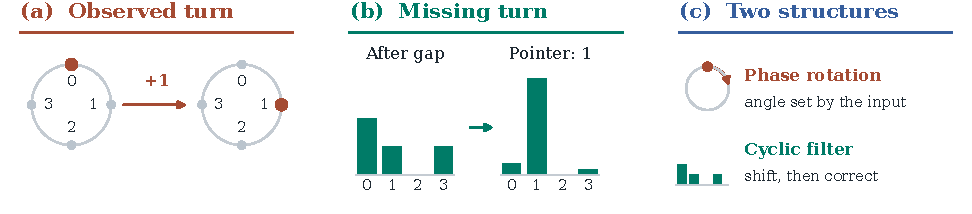
\includegraphics[width=\linewidth]{figures/overview_tracking.pdf}
\caption{From observations to actions in a four-position cycle.
(a) An observed turn moves the valve from position 0 to 1.
(b) An unrecorded turn leaves several possible positions. The bars show the
probability of each position before and after a noisy pointer reading of 1.
(c) The two structures we study: a phase rotation with its angle set by the
input, and a cyclic filter that shifts a belief and corrects it with a reading.}
\label{fig:overview}
\label{fig:method}
\end{figure}

This paper asks where a known cycle should enter a learned model.
Section~\ref{sec:method} describes two options. A \emph{phase rotation} builds the
cycle into the state update: the input sets a rotation angle, and a
squared-amplitude readout turns the rotated state into probabilities. A
\emph{cyclic filter} builds the cycle into the belief update instead: it shifts a
distribution over positions and then corrects it with a pointer reading.
Section~\ref{sec:exp} compares both structures with recurrent and attention
models in simulation, as the observations degrade from clean to noisy to
missing. To see whether a better belief also leads to better decisions, we give
every estimator's belief to the same planner. Beliefs are scored by the negative
log likelihood (NLL) of the true position, and control by net utility, the
success indicator minus the cost of turns and readings. Section~\ref{sec:imu}
then tests both structures on a recorded inertial sensor.

The answer depends on where the uncertainty enters. With clean events, letting
the input set the rotation angle is what allows a policy to learn the count from
a terminal reward. With noisy or missing events, the cyclic filters give the most
accurate beliefs, although a shared planner turns these better beliefs into
only small gains in net utility; the clearest effect is on whether the planner
takes another reading. On the recorded sensor, a rotation driven by the measured
gyroscope increment stays accurate far beyond its training length, whereas
recurrent and attention models given the same inputs do not. A classical filter
with bias estimation remains more accurate than all learned models.

\subsection{Related work}
\label{sec:related}

\myparagraph{Representing a cyclic state.}
Unitary RNNs and oscillatory recurrences use norm-preserving or undamped
dynamics \citep{arjovsky2016urnn,rusch2021cornn}. \citet{grazzi2025negative} give
an exact two-coordinate rotation and a linear template decoder for modular
counting. Our phase rotation uses the same input-dependent rotation as the
cyclic construction of \citet{karuvally2025aussm}, and
\citet{shakerinava2026diagonal} characterize the broader Abelian case for complex
diagonal state-space models. DeltaProduct tracks groups and extrapolates in
length through products of Householder updates \citep{siems2025deltaproduct}. We
use a small official-layer adapter, and its results apply to the tested width,
depth, and training recipe.

\myparagraph{Counting on longer sequences.}
Parity and modular counting are standard probes of length extrapolation
\citep{deletang2023chomsky}. Transformers can fit these tasks through
length-specific shortcuts \citep{liu2023shortcuts,zhou2024rasp}, and state-space
models and Transformers face expressivity limits on group word problems
\citep{merrill2024illusion}. Networks trained on modular arithmetic discover
Fourier features \citep{nanda2023grokking,chughtai2023universality,zhong2023clock},
and residue hyperdimensional computing combines unit-root codes by phasor
multiplication \citep{kymn2025residue}. We ask a different question: whether a model
can learn to count from a terminal reward, and how the answer changes when events
are noisy or missing.

\myparagraph{Memory and belief under partial observation.}
Recurrent policies are a standard baseline
\citep{hausknecht2015drqn,ni2022recurrent}. Reward machines provide automaton
memory learned from experience \citep{icarte2019reward}. Hidden actions and
occasional state reveals have been studied with probabilistic automata
\citep{siems2026code}. \citet{zhao2026belief} relate recurrent memory to belief
logits under deterministic transitions and extend their filters to
action-controlled settings. Born probabilities have also been used to
parameterize quantum-circuit policies \citep{jerbi2021parametrized}; our readout
is a classical squared amplitude. Unlike these works, we isolate the effect of a
belief on decisions by giving every estimate to the same planner.

\myparagraph{Inertial heading estimation.}
Complementary filters fuse gyroscope integration with gravity and magnetic
references \citep{mahony2008complementary}. VQF adds gyroscope bias estimation
and magnetic disturbance rejection \citep{laidig2023vqf}, and the BROAD benchmark
records these conditions with an optical reference \citep{laidig2021broad}. We
report both filters alongside the learned models.

\section{Related Work}\label{sec:related}

\myparagraph{Representing a cyclic state.}
Unitary RNNs and oscillatory recurrences use norm-preserving or undamped
dynamics \citep{arjovsky2016urnn,rusch2021cornn}. \citet{grazzi2025negative} give
an exact two-coordinate rotation with a linear template decoder for modular
counting. Our phase rotation uses the input-dependent rotation in the cyclic
construction of \citet{karuvally2025aussm}. \citet{shakerinava2026diagonal}
characterize complex diagonal state-space models for the broader Abelian case,
and DeltaProduct uses products of Householder updates to track group elements
\citep{siems2025deltaproduct}. Squared amplitudes also parameterize
quantum-circuit policies \citep{jerbi2021parametrized}. We show that a rotation
with a classical squared-amplitude readout learns exact tracking from terminal
reward by taking its angle directly from the observed increment.

\myparagraph{Counting on longer sequences.}
Parity and modular counting are standard probes of length extrapolation
\citep{deletang2023chomsky}. Transformers can fit these tasks through
length-specific shortcuts \citep{liu2023shortcuts,zhou2024rasp}, and state-space
models and Transformers face expressivity limits on group word problems
\citep{merrill2024illusion}. Networks trained on modular arithmetic can learn
Fourier features \citep{nanda2023grokking,chughtai2023universality,zhong2023clock},
and residue hyperdimensional computing combines unit-root codes by phasor
multiplication \citep{kymn2025residue}. We show that phase rotation extends
terminal-reward counting beyond the training lengths and that a categorical
count belief extends it to noisy event cues.

\myparagraph{Memory and belief under partial observation.}
Recurrent policies are a standard baseline for partially observed tasks
\citep{hausknecht2015drqn,ni2022recurrent}. \citet{ni2023transformers} separate
memory from credit assignment in evaluations of Transformer policies, and
POPGym benchmarks memory architectures under partial observation
\citep{morad2023popgym}. Reward machines learn automaton memory from experience
\citep{icarte2019reward}, and probabilistic automata model hidden actions and
occasional state reveals \citep{siems2026code}. \citet{lambrechts2022recurrent}
find that hidden states of RNNs trained for Q-learning correlate with the
decision-relevant part of the belief. \citet{zhao2026belief} relate recurrent
memory to belief logits under deterministic transitions and extend their filters
to action-controlled settings. We use a shared planner to show how more
accurate cyclic beliefs improve utility by changing the decision to sense.

\myparagraph{Differentiable Bayes filters.}
Differentiable filters retain the algorithmic structure of Bayesian prediction
and correction while learning parts of the update. Prior work has used
histogram and particle representations
\citep{jonschkowski2016histogram,jonschkowski2018dpf}, learned components of
Kalman filters \citep{haarnoja2016backprop,revach2022kalmannet}, and compared
training choices for differentiable filters \citep{kloss2021differentiable}.
QMDP-Net embeds filtering and planning in a policy
\citep{karkus2017qmdpnet}. Particle-based inference also appears in recurrent
networks and variational reinforcement learning
\citep{ma2020pfrnn,igl2018dvrl}. Our cyclic filter specializes the differentiable
histogram filter of \citet{jonschkowski2016histogram} to a known cyclic group
with exact shifts. We show that assigning probabilities to those shifts from
a learned token misread model brings its beliefs close to matched Bayes under
state supervision.

\myparagraph{Circular filtering and harmonic representations.}
Circular Bayesian filters use distributions defined directly on the circle
\citep{kurz2016circular}, and harmonic exponential families use Fourier
representations on manifolds \citep{cohen2015harmonic}. We show that a heading
belief updated by harmonic shifts and a learned pointer likelihood matches the
best neural tracking error under magnetic disturbance.

\myparagraph{Inertial heading estimation.}
RoNIN learns inertial navigation from IMU sequences \citep{herath2020ronin}.
TLIO fuses learned displacement estimates in a filter \citep{liu2020tlio},
and AI-IMU Dead-Reckoning learns to adapt filter noise parameters
\citep{brossard2020aiimu}. Complementary filters combine gyroscope integration
with gravity and magnetic references \citep{mahony2008complementary}. VQF adds
gyroscope bias estimation and magnetic disturbance rejection
\citep{laidig2023vqf}, and BROAD provides recordings with an optical orientation
reference \citep{laidig2021broad}. On BROAD we show that supplying the
integrated increment supports extrapolation across architectures and that a
bias state driven by physical rest detection reduces heading error further.

\FloatBarrier
\section{Problem Setting}\label{sec:setting}
\label{sec:prelim}
\label{sec:problem}

In the cyclic partially observable Markov decision process (POMDP), the latent
position is $s_t\in\Z_k$, with known cycle size $k$ and positions numbered from
$0$ to $k-1$ \citep{kaelbling1998pomdp}. The increment $j_t$ gives
$s_t=(s_{t-1}+j_t)\bmod k$. An observation $o_t\in\R^n$ can contain a cue about
$j_t$ and a pointer reading $y_t$ of the absolute position $s_t$. The agent can
choose an action $a_t$ after observing $o_t$. In control, actions can affect the
next increment or request a new pointer reading. The belief is the posterior
probability of each position,
\[
b_t(s)=\Pr(s_t=s\mid o_{1:t}),
\]
with past actions included in the observation history for controlled sequences.
A learned policy updates a memory $h_t=f_\phi(o_t,h_{t-1})$ and assigns action
probabilities $\pi_\phi(a\mid h_t)$.

We evaluate belief estimates beyond the training lengths using the accuracy of
the most probable position and the negative log likelihood (NLL) of the true
position, $-\log b_t(s_t)$. The fixed shared planner selects actions from each
estimator's belief to maximize expected net utility, defined as the success
indicator minus the costs of turns and readings
(Section~\ref{sec:regimes}).

\myparagraph{Counting tasks.}
In the \textbf{mod-$k$} task, each of the $L$ observations encodes a binary event
bit $e_t\in\{0,1\}$. A single decision at the final step earns $+1$ for the
correct count $a^\star=\big(\sum_{t=1}^{L} e_t\big)\bmod k$ and $-1$ otherwise.
Parity is the case $k=2$. Models train on a bounded range of lengths and are
evaluated on longer ones. On clean inputs, the programmed counter
$c_t=(c_{t-1}+e_t)\bmod k$ is an exact oracle. The experiment tests whether a
policy can learn the count from terminal reward. Two control tasks remove the
cyclic structure. In the \textbf{cue} task a single informative bit appears at
$t=1$. In the \textbf{monotone} task the agent reports whether the count exceeds
$L/2$. Sections~\ref{sec:transfer} and~\ref{sec:feedback} describe the valve
control and missing-event tasks.

\section{Two Cyclic Structures}
\label{sec:method}

\subsection{Tasks}
\label{sec:prelim}
\label{sec:problem}
At each step $t$ the agent receives an observation $o_t\in\R^n$, updates a
memory $h_t=f_\phi(o_t,h_{t-1})$, and assigns action probabilities
$\pi_\phi(a\mid h_t)$. The true position is one of $k$ positions on a known
cycle, and the memory may represent a single position or a probability over
several.

In the \textbf{mod-$k$} task, each of the $L$ observations encodes a binary event bit
$b_t\in\{0,1\}$. A single decision at the final step earns $+1$ if it equals the
running count $a^\star = \big(\sum_{t=1}^{L} b_t\big) \bmod k$ and $-1$ otherwise.
Parity is the case $k=2$. Models train on a bounded range of lengths and are
evaluated on longer ones. Two control tasks remove the cyclic structure: in the
\textbf{cue} task a single informative bit appears at $t=1$, and in the
\textbf{monotone} task the agent reports whether the count exceeds $L/2$. On
clean inputs, the programmed counter $c_t=(c_{t-1}+b_t)\bmod k$ is an exact
oracle, so the question is whether a policy can learn this counter from reward
alone. Sections~\ref{sec:transfer} and~\ref{sec:feedback} introduce the valve
and missing-event tasks.

\subsection{An input-conditioned phase rotation}
\label{sec:arch}
If the $k$ positions are marked around a circle, increasing the count by one
rotates a point by $2\pi/k$. We therefore keep a complex memory $z\in\C^d$ and,
at each step, rotate each coordinate by an angle chosen from the observation
before adding a learned input term:
\begin{equation}
z \;\leftarrow\; z \odot e^{\,i\,\theta(o_t)} \;+\; \mathrm{inj}(o_t),
\qquad \theta(o)=W_\theta\, o,
\label{eq:evolve}
\end{equation}
where $\odot$ denotes elementwise multiplication and $\theta(o)\in\R^d$ holds
the rotation angles. The rotation preserves each coordinate's magnitude, so $k$
advances of $2\pi/k$ return a coordinate exactly to its starting point; the
additive term $\mathrm{inj}(o)\in\C^d$ lets the observation change the
amplitudes as well. To read out an action, the model maps the state linearly to
one complex amplitude $\psi_a$ per action and normalizes the squared magnitudes.
We call this the Born readout:
\begin{equation}
\psi_a = \textstyle\sum_j w_{aj}\, z_j \in \C,
\qquad
\pi(a) = \frac{|\psi_a|^2}{\sum_b |\psi_b|^2}.
\label{eq:born}
\end{equation}
An all-zero score vector falls back to the uniform distribution, and sampling
floors probabilities at $10^{-8}$. When one coordinate stays fixed as a reference
and another rotates, the squared magnitude contains a term comparing their
phases, and this term peaks at the action aligned with the accumulated rotation.
Equivalently, the model is a real $SO(2)$ rotation with quadratic features.

\begin{proposition}[Exact and length-invariant representation;
cf.\ \citealp{grazzi2025negative,karuvally2025aussm}]
\label{prop:exact}
A parameter setting of Equations~\eqref{eq:evolve} and \eqref{eq:born} with width
$d=2$ makes the greedy action $\arg\max_a \pi(a)$ equal the true count $a^\star$ for
every length $L$ and every input sequence $b_1,\dots,b_L$.
\end{proposition}

The proof is in Appendix~\ref{app:proofs}. The proposition shows that exact
counting is representable; whether training finds such a setting is an empirical
question. A classical relative-phase score
$\operatorname{Re}(\overline{z_0}z_1\omega^{-a})$ selects the same action.
Appendix~\ref{app:proofs} also discusses the readout's global-phase invariance,
and Appendix~\ref{app:contractive} shows that uniformly contractive memories
cannot keep a positive decoding margin over long common suffixes.

\label{sec:stab}
\myparagraph{Training stabilizers and angular error.}
In the curriculum experiments we renormalize $z\leftarrow z/\lVert z\rVert_2$
after each step and add the penalty
$\lambda\langle\sin^2(\tfrac{k}{2}\theta(o_t))\rangle$ to pull angles toward
multiples of $2\pi/k$. Neither operation enforces exact angles, and a nonzero
injection can also shift the phase. For the two-channel construction without
injection, per-step phase errors of at most $\epsilon$ and an initial error $\epsilon_0$
give angular error at most $\eta=\epsilon_0+L\epsilon$ after $L$ steps. Nearest-residue
decoding stays correct for $\eta<\pi/k$, and with score perturbations of at most
$\delta$ it suffices that $\cos\eta-\cos(2\pi/k-\eta)>\delta$. Because the admissible error shrinks as $1/k$,
larger cycles are harder to track with a learned angle.

\subsection{A cyclic filter for uncertain increments}
\label{sec:filter}
A rotation carries a single count. Once an event may be missing or misread,
the model needs a probability for each position instead. Starting at zero, for
example, one missing turn leaves probability $0.50$ on position zero and $0.25$ on
each of positions one and three; a pointer reading of one then makes position one
more likely. A cyclic filter carries out these two steps as a prediction followed
by a correction:
\begin{align}
\tilde b_t &= \sum_{d} q_t(d)\, P_d\, b_{t-1},\label{eq:filter-predict}\\
b_t(s) &\propto \tilde b_t(s)\, \ell_t(y_t\mid s).\label{eq:filter-correct}
\end{align}
Here $P_d$ shifts the belief $b$ around the cycle by $d$ positions, a learned
event encoder supplies the probability $q_t(d)$ of each increment, and $\ell_t$
is the likelihood of the pointer reading $y_t$ at position $s$; without a reading,
$b_t=\tilde b_t$. Because the shifts are exact, only the event probabilities and
the pointer likelihood need to be learned. The categorical counter of
Section~\ref{sec:noisy} is the special case without pointer readings. For a
continuous increment $u_t$, the shift multiplies the belief's Fourier
coefficients by $e^{-inu_t}$, so the filter applies the phase rotation of
Section~\ref{sec:arch} to a whole distribution (Section~\ref{sec:imu}).

\section{Simulated Experiments}
\label{sec:exp}
\label{sec:setup}

The shaded cells in Table~\ref{tab:summary} mark the models that place
structure at the source of uncertainty. Each shaded model attains the best
value among the learned estimators shown, including ties.

\subsection{Clean events: learning to count from a terminal reward}
\label{sec:rl}
\label{sec:boundary}
We train policies with advantage actor-critic on clean sequences of length
10, using terminal reward as the training signal. Cue and monotone controls
test simpler memory tasks under the same setup.

At the common budget of $7.68$ million environment steps, four of five
phase-rotation seeds and one of five Transformer seeds reach the parity
threshold (Figure~\ref{fig:reward}a). On $\Z_3$, all five seeds of both
models reach the threshold, and phase rotation reaches both tasks'
thresholds sooner in median steps (Figure~\ref{fig:reward}b and
Table~\ref{tab:main}). After
training on lengths 4 through 14, phase rotation reaches $1.00$ on parity
and $0.90$ on $\Z_3$ at length 40.
\label{sec:lengthgen}
\begin{table}[tbp]
\centering\small
\caption{Learning from terminal reward on clean sequences of length 10.
Final success is the mean at the end of training over five seeds.
Crossing means reaching $0.90$ greedy success on parity or $0.70$ on $\Z_3$.
The median step count includes runs censored at their training budget
($7.68$M steps for GRU, LSTM, and Born, and $20.48$M for the Transformer).
The seed count uses the common budget of $7.68$M steps.}
\label{tab:main}
\begin{tabular}{llrrrr}
\toprule
Task & Measure & GRU & LSTM & Transformer & Born \\
\midrule
Cue & Final success & 1.00 & 1.00 & 1.00 & 1.00 \\
Monotone & Final success & 1.00 & 1.00 & 1.00 & 1.00 \\
\midrule
$\Z_2$ & Final success & .50 & .50 & .883 & .901 \\
      & Median crossing steps & $>$7.68M & $>$7.68M & 15.7M & 2.6M \\
      & Seeds crossing by $7.68$M & 0/5 & 0/5 & 1/5 & 4/5 \\
$\Z_3$ & Final success & .40 & .33 & .975 & .997 \\
      & Median crossing steps & $>$7.68M & $>$7.68M & 2.4M & 0.26M \\
      & Seeds crossing by $7.68$M & 0/5 & 0/5 & 5/5 & 5/5 \\
\bottomrule
\end{tabular}
\end{table}

Appendix~\ref{app:clean} gives the protocols and learning curves' summary
statistics.

\begin{figure}[!htbp]
\centering
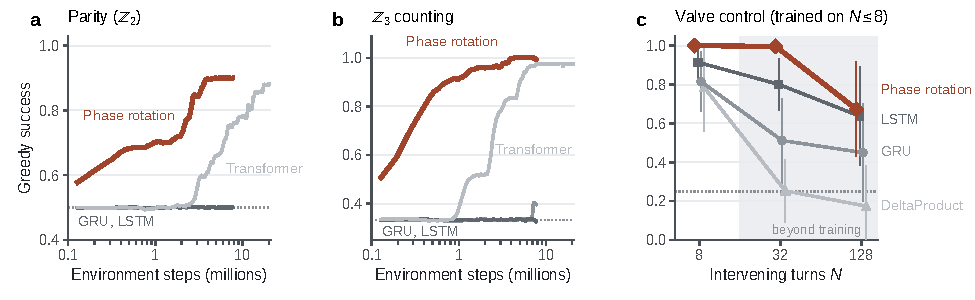
\includegraphics[width=\linewidth]{figures/fig_reward.pdf}
\caption{(a, b)~Greedy success on length-10 parity and $\Z_3$ counting is
plotted against millions of environment steps on a log scale for phase
rotation (337 and 369 parameters), the Transformer (5.9k, 20.48M-step budget),
the GRU (1.1k), and the LSTM (1.5k).
Curves show five-seed means with a five-point moving average.
(c)~Points and bars show five-seed means and sample SDs for valve success at
$N=8,32,128$ for phase rotation, the validation-selected LSTM ($H=16$) and
GRU ($H=64$), and the DeltaProduct adapter.
Dotted lines mark chance success, and shading in (c) marks horizons beyond
the training range $N\leq8$.}
\label{fig:reward}
\end{figure}

\myparagraph{The input-set angle.}
In a matched parity ablation, a diagonal complex recurrent model with a
fixed unit-modulus rotation and a squared-amplitude readout averages
$0.66$ accuracy at length 10. Setting the angle from the input raises
accuracy to $0.996$ at the same width and training budget
(Appendix~\ref{app:lru}). The input-conditioned model reaches $0.57$ at
length 20 without stabilizers. Normalization and the angle penalty target
accumulating angular error (Section~\ref{sec:stab}). Phase-advance and
readout ablations link the gains to the phase carried by the transition.
On frozen recurrent states, the squared-amplitude readout gives the
highest clean parity accuracy at length 80 (Appendix~\ref{app:clean-probes}).

\phantomsection
\myparagraph{Using the count to operate a valve.}
\label{sec:transfer}
In the four-position valve task, the policy sees the initial pointer and the
target, then receives cues for the intervening commands and their outcomes.
It makes corrective turns and selects the finish action. Training uses
1--8 intervening turns and terminal reward, and $N$ denotes the number of
intervening turns at evaluation.

The re-tuned comparison gives every family three times the original tuning
budget and a wider learning-rate grid, with a width sweep for the GRU and
LSTM. Phase rotation reaches $1.000$ success at $N=8$ and $0.997$ at $N=32$, four
times the longest training horizon, compared with $0.915$ and $0.801$ for
the best budget-matched baseline (Table~\ref{tab:valve}, Figure~\ref{fig:reward}c).
At $N=128$, sixteen times the longest training horizon, phase rotation
reaches $0.673$ and the best learned baseline reaches $0.684$. The
programmed counter succeeds at every horizon. Appendix~\ref{app:valve}
gives the tuning protocol and original-budget results.

\begin{table}[!htbp]
\centering\small
\caption{Re-tuned valve control after training on 1--8 intervening turns.
Greedy success is mean $\pm$ sample SD over five seeds, with 4,096
episodes per seed and horizon. LR is the validation-selected learning rate.}
\label{tab:valve}
\setlength{\tabcolsep}{4pt}
\begin{tabular}{@{}llrrrr@{}}
\toprule
Memory type & Policy & LR & $N=8$ & $N=32$ & $N=128$ \\
\midrule
Phase rotation & Phase rotation ($H=16$) & 0.003 & \textbf{1.000}\,$\pm$\,0.000 & \textbf{0.997}\,$\pm$\,0.005 & 0.673\,$\pm$\,0.244 \\
\midrule
\multirow{6}{*}{Gated recurrence} & LSTM ($H=16$) & 0.01 & 0.915\,$\pm$\,0.106 & 0.801\,$\pm$\,0.136 & 0.637\,$\pm$\,0.253 \\
 & LSTM ($H=32$) & 0.01 & 0.796\,$\pm$\,0.269 & 0.735\,$\pm$\,0.249 & \textbf{0.684}\,$\pm$\,0.284 \\
 & LSTM ($H=64$) & 0.003 & 0.669\,$\pm$\,0.228 & 0.633\,$\pm$\,0.183 & 0.559\,$\pm$\,0.157 \\
 & GRU ($H=16$) & 0.003 & 0.344\,$\pm$\,0.102 & 0.291\,$\pm$\,0.121 & 0.285\,$\pm$\,0.122 \\
 & GRU ($H=32$) & 0.01 & 0.737\,$\pm$\,0.205 & 0.379\,$\pm$\,0.099 & 0.296\,$\pm$\,0.101 \\
 & GRU ($H=64$) & 0.01 & 0.815\,$\pm$\,0.156 & 0.512\,$\pm$\,0.219 & 0.450\,$\pm$\,0.253 \\
\midrule
State-tracking layer & DeltaProduct adapter ($H=16$) & 0.003 & 0.784\,$\pm$\,0.228 & 0.253\,$\pm$\,0.163 & 0.174\,$\pm$\,0.208 \\
\midrule
Categorical & Learned cyclic counter ($H=16$) & 0.003 & 0.553\,$\pm$\,0.109 & 0.549\,$\pm$\,0.113 & 0.552\,$\pm$\,0.119 \\
\bottomrule
\end{tabular}
\end{table}


\subsection{One protocol, rising uncertainty}
\label{sec:sweep}
We start from an exact pointer on a four-position valve, then replace each
delivered turn token with a uniformly drawn alternative with probability $r$.
The increments regime delivers every token, while the missing regime erases
bursts and supplies noisy pointer readings.

Each learned model trains at the test misread rate on lengths $6$, $10$,
and $14$ for 3{,}000 Adam updates with batch size 96 and gradient clipping
at norm 1. Two tuning seeds evaluate the learning-rate grid
$\{10^{-3},3\times 10^{-3},10^{-2}\}$. Validation NLL selects the rate
for dense and terminal labels, and validation accuracy selects it for
terminal reward. We report final-state NLL and accuracy over five test
seeds and 1{,}024 episodes per seed and cell.

Table~\ref{tab:sweep} compares the training signals at $L=40$. On clean
inputs with a terminal label or reward, the measured-angle rotation and
the cyclic filters reach $1.000$ accuracy through $L=160$, while the GRU,
LSTM, and learned-angle rotation stay at chance.

\begin{table}[!htbp]
\centering\small
\caption{Increments regime at $L=40$. Each cell gives mean terminal
NLL (nats) / accuracy over five test seeds. Appendix~\ref{app:sweep}
reports the full sweep and NLL standard deviations.}
\label{tab:sweep}
\setlength{\tabcolsep}{3pt}
\begin{tabular}{@{}lrrrrrr@{}}
\toprule
& \multicolumn{3}{c}{$r=0$} & \multicolumn{3}{c}{$r=0.01$} \\
\cmidrule(lr){2-4}\cmidrule(l){5-7}
Estimator & Dense & Terminal & Reward & Dense & Terminal & Reward \\
\midrule
GRU & $0.000\,/\,1.000$ & $1.386\,/\,0.255$ & $7.503\,/\,0.255$ & $1.062\,/\,0.682$ & $1.387\,/\,0.251$ & $7.510\,/\,0.252$ \\
LSTM & $0.000\,/\,1.000$ & $1.386\,/\,0.255$ & $1.634\,/\,0.250$ & $1.159\,/\,0.679$ & $1.386\,/\,0.257$ & $1.937\,/\,0.242$ \\
Phase rotation (learned angle) & $0.003\,/\,1.000$ & $1.387\,/\,0.255$ & $2.418\,/\,0.244$ & $1.412\,/\,0.417$ & $1.387\,/\,0.252$ & $2.365\,/\,0.244$ \\
Phase rotation (measured angle) & $0.000\,/\,1.000$ & $0.000\,/\,1.000$ & $0.002\,/\,1.000$ & $1.309\,/\,0.683$ & $1.161\,/\,0.683$ & $2.494\,/\,0.683$ \\
Cyclic filter (token-constrained) & $0.000\,/\,1.000$ & $0.000\,/\,1.000$ & $0.000\,/\,1.000$ & $5.839\,/\,0.683$ & $5.839\,/\,0.683$ & $5.839\,/\,0.683$ \\
Cyclic filter (unconstrained) & $0.000\,/\,1.000$ & $0.000\,/\,1.000$ & $0.002\,/\,1.000$ & $0.967\,/\,0.683$ & $0.971\,/\,0.683$ & $2.379\,/\,0.683$ \\
Cyclic filter (misread-aware) & $0.012\,/\,1.000$ & $0.011\,/\,1.000$ & $0.314\,/\,1.000$ & $0.966\,/\,0.683$ & $0.966\,/\,0.683$ & $0.972\,/\,0.683$ \\
\midrule
Matched Bayes & $0.000\,/\,1.000$ & $0.000\,/\,1.000$ & $0.000\,/\,1.000$ & $0.965\,/\,0.683$ & $0.965\,/\,0.683$ & $0.965\,/\,0.683$ \\
\bottomrule
\end{tabular}
\end{table}


At $r=0.01$ and $L=40$, the token-constrained filter matches Bayes in
accuracy. Its NLL rises because it treats reported shifts as certain and
assigns near-zero probability to the true position if misreads change the
final residue. We floor probabilities at $10^{-8}$ for NLL. The misread-aware
filter reaches terminal-label NLL of $0.966$, compared with $5.839$ for
the token-constrained filter and $0.965$ for matched Bayes
(Figure~\ref{fig:sweep}a). With missing tokens and noisy readings at $r=0.3$
and $L=160$, it matches Bayes at $1.263$ NLL under state labels and leads
the learned models at $1.637$ under reward (Figure~\ref{fig:sweep}c).
Appendix~\ref{app:sweep} gives the full sweep.

\begin{figure}[!htbp]
\centering
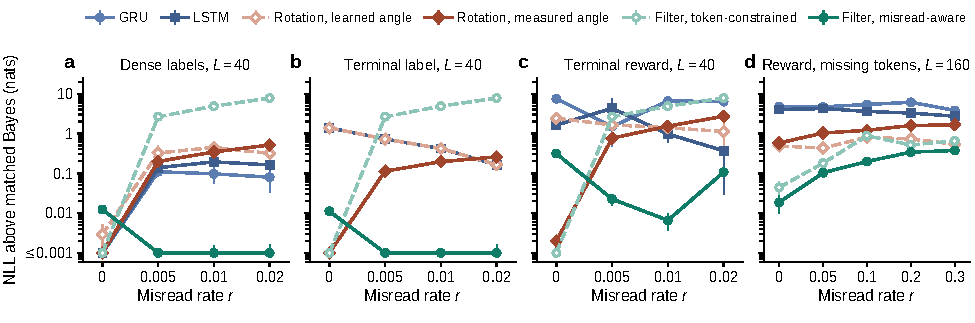
\includegraphics[width=\linewidth]{figures/fig_sweep.pdf}
\caption{Excess test NLL over matched Bayes versus token misread rate $r$.
(a, b)~The increments regime uses a terminal label and terminal reward,
respectively, at $L=40$, and (c) uses terminal reward with missing tokens
and pointer readings at $L=160$.
Points and bars show the mean and sample SD of NLL differences paired across
five test seeds, with values below $0.001$ nats at the floor of the log axis.
The thick line marks the misread-aware filter, the dashed line with open
markers marks the token-constrained filter, and grey lines show the GRU and
LSTM.}
\label{fig:sweep}
\end{figure}

\subsection{Noisy events: inferring the event before counting}
\label{sec:noisy}
We replace the observed bit with a 16-dimensional Gaussian feature vector.
The learned cyclic counter predicts event probabilities and mixes exact
shifts of the count belief. It reaches $0.994$ accuracy at $L=160$ for
$k=2,3,4$ (Table~\ref{tab:noisy}).

A learned-angle rotation represents each noisy cue by a single angle.
The cue can support multiple events, so a wrong increment shifts the
estimate and later updates accumulate these errors. With an angle penalty,
accuracy approaches chance by length 40 for $k=2,3$. At $k=4$ and $L=160$,
enforcing exact multiples of $2\pi/k$ raises accuracy from $0.248$ to
$0.562$, compared with $0.756$ for the width-32 LSTM. The cyclic counter
carries event uncertainty forward by assigning probabilities to the
possible shifts.

\begin{table}[!t]
\centering\small
\caption{Counting with noisy event features: greedy accuracy at the longest
training length ($L=14$) and at $L=160$, mean (SD) over five seeds. Chance is
$1/k$. Appendix~\ref{app:additional} reports all lengths and further baselines.}
\label{tab:noisy}
\setlength{\tabcolsep}{4pt}
\begin{tabular}{lcccccc}
\toprule
& \multicolumn{2}{c}{$k=2$} & \multicolumn{2}{c}{$k=3$} & \multicolumn{2}{c}{$k=4$} \\
\cmidrule(lr){2-3}\cmidrule(lr){4-5}\cmidrule(lr){6-7}
Model & $L=14$ & $L=160$ & $L=14$ & $L=160$ & $L=14$ & $L=160$ \\
\midrule
Cyclic counter & \textbf{.999} (.001) & \textbf{.994} (.002) & \textbf{.999} (.001) & \textbf{.994} (.002) & \textbf{.999} (.001) & \textbf{.994} (.002) \\
LSTM, width 32 & .947 (.113) & .933 (.118) & .967 (.071) & .944 (.075) & .765 (.345) & .756 (.338) \\
Born, hard angles & .492 (.021) & .499 (.015) & .841 (.283) & .699 (.214) & .884 (.079) & .562 (.081) \\
Born, soft penalty & .701 (.048) & .503 (.009) & .719 (.019) & .335 (.010) & .689 (.092) & .248 (.008) \\
\bottomrule
\end{tabular}
\end{table}


\subsection{Missing events: estimating the belief}
\label{sec:feedback}
We train estimators on four-position valve histories with a state label at
each step. Visible tokens give the exact turn, and occasional noisy pointer
readings correct the belief during histories with missing turns. The
token-constrained filter uses the known shift on visible turns, and the
unconstrained filter learns shift probabilities on every step.

On test histories with four consecutive missing turns and a pointer every
twelve steps, the token-constrained filter reaches $0.937$ NLL, compared with
$0.982$ for phase rotation and $1.011$ for the GRU. Both cyclic filters
achieve near-zero circular regret. At length 80, the token-constrained
filter's NLL falls from $1.361$ immediately before a reading to $0.591$
at the reading.

Table~\ref{tab:feedback} compares estimation and default-planner utility
on the same histories. Nominal Bayes uses the training parameters, and
matched Bayes uses the test parameters. Both compute posteriors from the
same observations as the learned estimators. The tests include shifts in
turn probabilities and pointer reliability. The token-constrained filter
comes within $0.0168$ nats of matched Bayes and gives lower NLL than
nominal Bayes ($0.937$ versus $0.944$).

\begin{table}[!htbp]
\centering\small
\caption{Cyclic filters give the lowest NLL and highest shared-planner utility
among learned estimators. The table averages five seeds, lengths 40 and 80, and the nominal,
event-rate shift, and pointer-noise shift conditions. Each history has four-step
bursts of missing turns and a pointer every twelve steps. Utility is scaled to
100 points. The last two columns give paired differences from matched Bayes
(mean $\pm$ sample SD). Circular regret is excess expected distance relative
to the best point estimate under matched Bayes.}
\label{tab:feedback}
\setlength{\tabcolsep}{2.7pt}
\begin{tabular}{llrccccrr}
\toprule
& & & \multicolumn{3}{c}{Estimation} & Control
& \multicolumn{2}{c}{Gap to matched Bayes} \\
\cmidrule(lr){4-6}\cmidrule(lr){7-7}\cmidrule(lr){8-9}
Prior & Estimator & Params & Acc.\,$\uparrow$ & NLL\,$\downarrow$
& Regret\,$\downarrow$ & Utility (pts) & $\Delta$NLL & $\Delta$Utility (pts) \\
\midrule
None & GRU & 1,844 & .634 & 1.011 & .0053 & 62.3
& $+.091\pm.006$ & $-1.05\pm0.48$ \\
Phase rotation & \shortstack[l]{Squared-amplitude\\readout} & 1,088 & .623 & .982 & .0067 & 62.3
& $+.061\pm.038$ & $-1.01\pm0.57$ \\
\midrule
\multirow{2}{*}{Cyclic filter} & Unconstrained & 196 & .634 & .938 & .0000 & 62.9
& $+.018\pm.003$ & $-0.46\pm0.32$ \\
& Token-constrained & 196 & .634 & \textbf{.937} & \textbf{.0000} & \textbf{63.0}
& $\mathbf{+.017\pm.002}$ & $\mathbf{-0.36\pm0.46}$ \\
\midrule
\multirow{2}{*}{Exact Bayes} & Nominal & 0 & .634 & .944 & .0000 & 62.7
& $+.024\pm.003$ & $-0.63\pm0.38$ \\
& Matched (ref.) & 0 & .641 & .920 & .0000 & 63.3 & --- & --- \\
\bottomrule
\end{tabular}
\end{table}


\subsection{Acting on the belief with a shared planner}
\label{sec:regimes}
The planner starts from each estimator's final belief and a target. It
chooses a turn, a pointer reading, or the finish action to maximize success
minus action costs. We vary the horizon, reading cost, and reading reliability
with the estimators fixed.

In the default setting, the token-constrained filter reaches $63.0$ utility
points, compared with $62.3$ for both the GRU and phase rotation, $62.7$
for nominal Bayes, and $63.3$ for matched Bayes (Table~\ref{tab:feedback}).
Both cyclic filters match or exceed the GRU in all
75 settings, with a positive paired bootstrap interval for the constrained
filter in 47 (Figure~\ref{fig:regimes}). Both retain at least $95\%$ of the
attainable gain in settings with at least ten points of headroom. The
differences in belief primarily affect the choice to read the pointer.
Appendix~\ref{app:regimes} gives the planner grid and sensing comparisons.

\begin{figure}[!htbp]
\centering
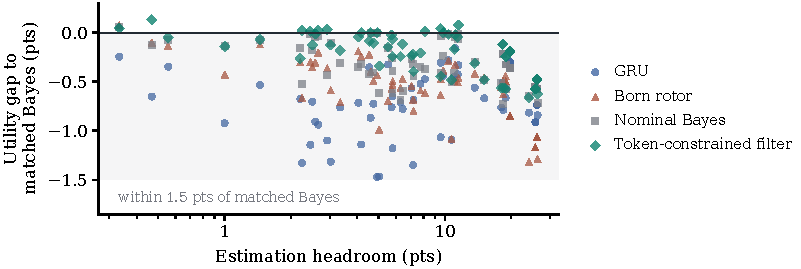
\includegraphics[width=\linewidth]{figures/fig_regimes.pdf}
\caption{Utility across 75 planner regimes, each averaged over six test
conditions and five seeds.
(a)~For the GRU, phase rotation, and the token-constrained filter in each
headroom group, the dot and bar show the median and interquartile range of
retained share across regimes.
Headroom is the utility gain of matched Bayes over a uniform belief, grouped
as below 3 points (12 regimes), 3 to under 10 points (23), and at least 10
points (40).
Dashed and dotted lines mark $100\%$ and $95\%$ retained, respectively.
(b)~The token-constrained filter's mean gain over the GRU is plotted against
headroom on a log scale with 95\% paired seed-bootstrap intervals, with filled
points for the 47 intervals above zero and open points for the 28 intervals
including zero.}
\label{fig:regimes}
\end{figure}

Cheap, reliable readings make the sensing decision sensitive to belief quality.
An overconfident belief lowers the estimated value of taking a reading. With a
two-action horizon, a $0.02$ reading cost, and reliability $0.95$, the GRU
belief leads to $0.64$ readings per episode, compared with $0.84$ for matched
Bayes. The cyclic filters preserve sensing utility across the grid. The GRU
falls below the uniform-belief baseline in three settings, by up to $0.92$
percentage points.

\section{Heading from a Recorded Inertial Sensor}
\label{sec:imu}

The heading of a moving sensor is a cyclic state with a continuous position. A
gyroscope measures a noisy increment of this state at every step, while a
magnetometer acts as a pointer reading that magnetic disturbances can corrupt. We
test both cases on BROAD, a public benchmark of 39 trials recorded with an
inertial measurement unit (IMU) and optical motion capture
\citep{laidig2021broad}. The motion capture provides only the labels and never
enters a model input. The protocol was fixed before training, and Appendix~\ref{app:imu}
records every later amendment.

\begin{figure}[!t]
\centering
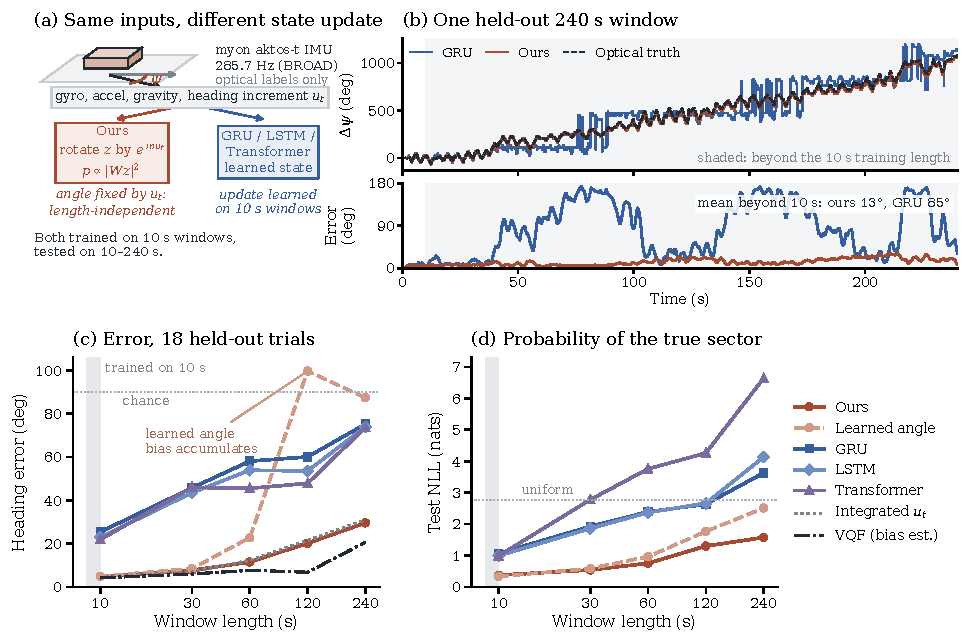
\includegraphics[width=\linewidth]{figures/imu_main.pdf}
\caption{Heading from a recorded IMU (BROAD, myon aktos-t at 285.7~Hz;
\citealp{laidig2021broad}). (a)~All learned models receive the same inputs; ours
sets its rotation angle from the measured increment $u_t$, while the GRU, LSTM,
and Transformer learn their state update. Every model trains on 10~s windows.
(b)~A held-out 240~s window from trial~20 (seed~0): heading change of each
model's most probable sector against the optical truth, and the error (2~s moving
average). (c)~Error at the window end and (d)~test NLL on 18 held-out trials,
averaged over five seeds and then trials. Gray curves are classical filters and
have no NLL. The 240~s windows come from the three longest test trials.}
\label{fig:imu}
\label{fig:imu-sensor}
\end{figure}

\subsection{Observed increments: gyroscope heading}
\label{sec:imu-gyro}
The first task is to estimate the heading change since the start of a window,
binned into 16 sectors of $22.5^\circ$. At 28.6~Hz, every learned model receives
the same inputs (Figure~\ref{fig:imu}a): the gyroscope and accelerometer readings, the gravity direction
from a causal complementary filter \citep{mahony2008complementary}, and that
filter's heading increment $u_t$. Models train on 10~s windows from 18 trials and
are tested on windows of 10 to 240~s from 18 other trials. In our model the input
sets the rotation angle, $\theta_t=n\,u_t$ for harmonics $n=1,\dots,8$, and a Born
readout (Equation~\eqref{eq:born}) turns the rotated state into sector
probabilities; only the readout and the initial phase are learned. A second
variant also learns a correction to the angle. The GRU, LSTM, and Transformer use
the same input encoder and more parameters.

Figure~\ref{fig:imu} summarizes the results. Panel~(b) shows one held-out
window: past the 10~s training length, our model keeps following the optical
heading, while the GRU repeatedly loses it by up to $180^\circ$. Across all test
trials (panels c and d), at every window length the input-set rotation has the lowest error and NLL of all learned models. At 240~s
its heading error is $29.6^\circ$, against $73.7^\circ$ for the best recurrent or
attention model, a paired difference of $-44.1^\circ$ with trial-bootstrap
interval $[-65.5,-31.4]$; the intervals exclude zero at all five lengths for both
error and NLL. The variant with a learned angle correction keeps pace up to 30~s
and then drifts. Its mean correction of $4.4\times10^{-4}$~rad per step is too
small to identify from 10~s windows, yet it accumulates to about $87^\circ$ at
120~s, consistent with the linear growth of angular error bounded in
Section~\ref{sec:stab}. The input-set rotation, in contrast, stays within
$1.4^\circ$ of integrating $u_t$ directly, so it keeps the accuracy of the
physical integrator while adding calibrated sector probabilities. It has no
bias state, however, and VQF, a filter that also estimates gyroscope bias
\citep{laidig2023vqf}, is more accurate from 30~s on and reaches $20.7^\circ$ at
240~s.

\subsection{Pointer readings: magnetometer under disturbance}
\label{sec:imu-mag}
The second task is to estimate the absolute heading in 64 sectors from a uniform
prior, with the tilt-compensated magnetometer heading added at every step as a
pointer reading. Five of the test trials contain recorded magnetic disturbances.
Our cyclic filter (Section~\ref{sec:filter}) shifts a categorical belief by $u_t$
through a phase rotation of its Fourier coefficients and corrects it with a
learned pointer likelihood. Its tracking error matches that of the best neural
network: on disturbed trials at 60~s, the difference from the LSTM is
$-1.4^\circ$ with interval $[-3.4,0.6]$. On undisturbed trials it beats a tuned
complementary filter by $1.2^\circ$ $[-2.1,-0.3]$, but its NLL is higher than that
of the GRU and LSTM. VQF, with its magnetic disturbance rejection, tracks within
$3.4^\circ$ on disturbed trials, against $9.5^\circ$ for our filter, and the
criterion we fixed in advance for this task is not met (Appendix~\ref{app:imu},
Table~\ref{tab:imu-b}).

Both tasks agree with the simulated results. When uncertainty enters through the
increments, fixing the transition to a rotation by the measured increment
generalizes from 10~s to 240~s, and unconstrained sequence models do not. When it
enters through a corrupted pointer, the useful structure lies in the pointer
model: our learned likelihood does not supply it, and the engineered disturbance
rejection in VQF does.

\FloatBarrier
\section{Discussion and Conclusion}
\label{sec:discussion}
\label{sec:conclusion}

When every turn is observed, an input-dependent rotation can represent an exact
count, and a policy can learn it from a terminal reward. A learned rotation angle,
however, accumulates small errors over time, and a categorical counter avoids
them by fixing each shift and weighting the shifts by event probabilities. When
turns are missing, a cyclic filter keeps several possible positions and updates
their probabilities whenever a pointer reading arrives. In our tests the cyclic
filters gave the most accurate beliefs among the learned models. Because the same
planner often chose the same action from different beliefs, these better beliefs
changed net utility by only about one point. Their clearest effect was on whether
to take another reading: when readings were cheap and reliable, an overconfident
estimate could lead the planner to skip a useful one.

These comparisons are controlled in three ways. We supply the cycle size, and in
the feedback study we train estimators with state labels and give the planner the
simulator's actuator and sensor models. A programmed counter shows what is
possible when every event is known, and a Bayes filter on the observed history
shows how much uncertainty remains when the observation model is known. Giving
every estimate to the same planner then tests whether better beliefs change
actions or costs. On real sensors, learning a bias state and a disturbance-aware
pointer model would be the next step toward the classical filter.

The recorded inertial sensor shows the same pattern outside simulation. A rotation
set by the measured heading increment kept its accuracy from 10~s training
windows to 240~s test windows, whereas recurrent and attention models given the
same inputs did not. Under magnetic disturbance our learned pointer model only
matched these networks, and an engineered filter with bias estimation and
disturbance rejection remained more accurate in both tasks. Taken together, the
results suggest that a known cycle helps most when it fixes the entry point of
uncertainty: the transition when increments are measured, and the pointer model
when readings are corrupted.


\bibliography{references}
\bibliographystyle{tmlr}

\clearpage
\appendix
\renewcommand{\thefigure}{S\arabic{figure}}
\renewcommand{\thetable}{S\arabic{table}}
\setcounter{figure}{0}
\setcounter{table}{0}
\renewcommand{\theHfigure}{appendix.\arabic{figure}}
\renewcommand{\theHtable}{appendix.\arabic{table}}
\section{Properties of the Phase Readout}
\label{app:proofs}

\myparagraph{Proof of Proposition~\ref{prop:exact}.}
\begin{proof}
Set $\omega = e^{2\pi i/k}$, $z_0=z_1=1$ initially, $\theta_0(o)=0$,
$\theta_1(o)=\tfrac{2\pi}{k}\,e(o)$ and $\mathrm{inj}\equiv 0$, with $e(o)$ the
event bit encoded in $o$. Then $z_0=1$ at every step and $z_1=\omega^{c}$ with
$c=\sum_t e_t$. Readout weights $w_{a0}=1$ and $w_{a1}=\omega^{-a}$ give
\begin{equation}
\psi_a = 1 + \omega^{\,c-a},\qquad
|\psi_a|^2 = 2 + 2\cos\!\Big(\tfrac{2\pi}{k}(c-a)\Big),
\label{eq:interference}
\end{equation}
maximized exactly at $a\equiv c \pmod{k}$. Normalizing the state multiplies the
two coordinates by the same positive scalar and leaves the maximizing action
unchanged.
\end{proof}


\begin{proposition}[Global-phase invariance of squared-amplitude scores]
\label{prop:gauge}
With the complex-linear convention $\psi_a=\sum_jw_{aj}z_j$, the score
$|\psi_a|^2$ is unchanged by $z\mapsto e^{i\varphi}z$.
No nonzero real-linear scalar score on $(\operatorname{Re}z,\operatorname{Im}z)$ has this
invariance, and the minimum degree of a nonconstant invariant real polynomial in these
coordinates is two.
\end{proposition}
\begin{proof}
Multiplying $z$ by $e^{i\varphi}$ multiplies $\psi_a$ by the same unit-modulus scalar.
Invariance under $\varphi=\pi$ forces any real-linear invariant to be zero, while
$\operatorname{Re}(\overline{z_i}z_j)$ gives a nonconstant quadratic invariant.
\end{proof}
Relative-phase cosine decoders and Hermitian quadratic forms also have this
symmetry, as do some nonpolynomial functions.
A fixed reference channel also permits exact real-linear decoding of the phase channel,
so absolute-phase controls compare information access as well as readout form.

\begin{lemma}[Phase blindness of magnitude-only readouts]
\label{lem:blind}
In the solution of Proposition~\ref{prop:exact}, the unit-modulus coordinate
$z_1=\omega^{c}$ carries the count and $|z_0|=|z_1|=1$. Any readout depending on the
coordinate magnitudes alone, $\pi(a)=f_a(|z_0|,|z_1|)$, is independent of $c$. Its accuracy
cannot exceed that of the best constant predictor, $\max_a \Pr[a^\star=a]$. This bound
equals the chance value $1/k$ exactly for a uniform residue, as in parity.
\end{lemma}

\begin{proof}
Along the solution $|z_0|=|z_1|=1$ for every input and every $c$, so $f_a(|z_0|,|z_1|)$ does not
depend on $c$ and induces a fixed action distribution $q(a)$. Its expected accuracy is
$\sum_a q(a)\,\Pr[a^\star=a]\le \max_a \Pr[a^\star=a]$. For independent uniform bits and $k=2$ the
residue is uniform, so the bound is the chance value $1/2$; more generally the bound equals $1/k$ precisely for a uniform residue distribution.
\end{proof}

Equation~\eqref{eq:interference} is a correlation with the first Fourier
character of the cycle. Using all $k$ characters would give the squared
magnitudes of the discrete Fourier transform.

\begin{proposition}[Zero set of the phase regularizer]
\label{prop:reg}
The regularizer $R(\theta)=\big\langle\sin^2\!\big(\tfrac{k}{2}\,\theta(o)\big)\big\rangle\ge 0$
(with $\langle\cdot\rangle$ the average over observations) satisfies $R(\theta)=0$ if and only if
$\theta(o)\in\tfrac{2\pi}{k}\Z$ for every observation in a finite average (or almost surely for an expectation); its zero set consists exactly of the
per-event rotations $\theta=2\pi j/k$ for $j\in\{0,\dots,k-1\}$. Among these, every $j$ with
$\gcd(j,k)=1$ is a faithful generator that yields an exact decoder by Proposition~\ref{prop:exact}
after relabeling actions $a\mapsto ja\bmod k$, while $j=0$ is a constant phase that cannot represent
counting. The canonical choice is the generator $j=1$, that is $\theta=2\pi/k$.
\end{proposition}

\begin{proof}
$\sin^2(\tfrac{k}{2}\theta)=0$ if and only if $\tfrac{k}{2}\theta\in\pi\Z$, that is
$\theta\in\tfrac{2\pi}{k}\Z$, with representatives $\theta=2\pi j/k$ in $[0,2\pi)$ for
$j=0,\dots,k-1$. Under such a rotation the phase channel after $c$ events is $\omega^{\,jc}$. The
map $c\bmod k\mapsto jc\bmod k$ is a bijection if and only if $\gcd(j,k)=1$, and the readout of
Proposition~\ref{prop:exact} then decodes $c$ after the stated relabeling. For $j=0$ the phase
is constant and phase-blind by Lemma~\ref{lem:blind}.
\end{proof}

The degenerate zero at $j=0$ explains an empirical sensitivity: the coefficient $\lambda$ must be
small enough that the reward objective keeps the rotation away from the no-rotation basin.

\section{Extrapolation across group orders}
\label{app:kboundary}
Table~\ref{tab:kscaling} reports reward-trained extrapolation after a
curriculum of lengths 4 through 14. The decoder margin below quantifies how
closely the ideal scores are spaced as $k$ increases. Controls with exact angles
are reported in Appendix~\ref{app:additional}.

\begin{lemma}[Interference margin and its decay in $k$]
\label{lem:margin}
In the exact solution of Proposition~\ref{prop:exact}, the squared-amplitude
score of the correct residue exceeds that of every other action by
\begin{equation}
\begin{aligned}
\Delta_k &\;=\; |\psi_{a^\star}|^2 - \max_{a\neq a^\star}|\psi_a|^2\\
&\;=\; 4 - \Big(2+2\cos\tfrac{2\pi}{k}\Big) \;=\; 4\sin^2\!\tfrac{\pi}{k}.
\end{aligned}
\label{eq:margin}
\end{equation}
The margin decays as $4\pi^2/k^2$ for large $k$.
\end{lemma}

\begin{proof}
From Equation~\eqref{eq:interference}, $|\psi_a|^2=2+2\cos(\tfrac{2\pi}{k}(c-a))$, maximal at $a=c$
with value $4$; the nearest competitors $a=c\pm1$ give $2+2\cos\tfrac{2\pi}{k}$. Subtracting and
using $1-\cos\theta=2\sin^2(\theta/2)$ gives
$\Delta_k=2\big(1-\cos\tfrac{2\pi}{k}\big)=4\sin^2\tfrac{\pi}{k}$; the small-angle expansion yields
the $O(1/k^2)$ decay.
\end{proof}


\begin{table}[tbp]
\centering
\caption{Zero-shot greedy accuracy at three evaluation lengths (five seeds; training curriculum
$L\in\{4,6,\dots,14\}$). Bold marks the higher accuracy of the two models.}
\label{tab:kscaling}
\small
\setlength{\tabcolsep}{3.5pt}
\begin{tabular}{cc ccc ccc}
\toprule
 & & \multicolumn{3}{c}{\textbf{Phase rotation}} & \multicolumn{3}{c}{LSTM} \\
\cmidrule(lr){3-5} \cmidrule(lr){6-8}
$k$ & chance & L10 & L40 & L80 & L10 & L40 & L80 \\
\midrule
\wsrow $2$ & 0.50 & \textbf{1.00} & \textbf{1.00} & \textbf{0.99} & 0.50 & 0.50 & 0.50 \\
\wsrow $3$ & 0.33 & \textbf{0.91} & \textbf{0.90} & \textbf{0.70} & 0.47 & 0.43 & 0.43 \\
$4$ & 0.25 & 0.80 & 0.55 & 0.54 & \textbf{0.88} & \textbf{0.85} & \textbf{0.84} \\
$5$ & 0.20 & 0.82 & 0.57 & 0.57 & \textbf{0.84} & \textbf{0.84} & \textbf{0.84} \\
\bottomrule
\end{tabular}
\end{table}


\section{Contraction, Margin, and Stochastic Decoding}
\label{app:contractive}
Norm preservation avoids one source of lost separability. The following result makes
this precise for uniformly contractive memories.

\begin{proposition}[Contraction and robust decoding]
\label{prop:contractive}
Suppose the state update is uniformly $\gamma$-contractive in its state, $0\le\gamma<1$.
If two prefixes produce states at distance at most $D$, appending a common suffix of
length $T$ leaves their states at distance at most $D\gamma^T$. If their target labels
differ and every decoder score is $K$-Lipschitz, the two predictions cannot both have a
correct-label margin $m>0$ once $KD\gamma^T<m$. For a balanced family of $k$ prefixes
carrying all residues, with state diameter at most $D$ and a common suffix, a stochastic
decoder with $K$-Lipschitz probability coordinates has mean success at most
$1/k+KD\gamma^T$.
\end{proposition}

\begin{proof}
Repeated contraction gives $\|h_T-h_T'\|\leq D\gamma^T$. If the two
correct labels are $a$ and $b$, both predictions having margin $m$ would
require $(s_a-s_b)(h_T)-(s_a-s_b)(h_T')\geq2m$. The difference of the
scores is $2K$-Lipschitz, so this requires $m\leq KD\gamma^T$.

For the balanced family, compare each terminal state $h_T^{(r)}$ to the
reference $h_T^{(0)}$. The correct labels $a_r$ are a permutation of the
$k$ residues, so the mean sampled success is bounded by
\[
\frac{1}{k}\sum_r p_{a_r}(h_T^{(r)})
\leq \frac{1}{k}\sum_r p_{a_r}(h_T^{(0)})+KD\gamma^T
= \frac{1}{k}+KD\gamma^T.
\]
\end{proof}
A contractive update can still decode with a vanishing margin. For example,
$h_0=1$ and $h_t=\gamma(-1)^{e_t}h_{t-1}$ recover parity by
$\arg\max(h_T,-h_T)$ at every finite length in exact arithmetic.

\section{The Diagonal Complex State-Space Baseline}
\label{app:lru}
We compare linear recurrent units (LRUs) on length-10 parity over five
seeds using the same width of 16, trainer, and budget as Table~\ref{tab:mech}.
Following \citet{orvieto2023lru}, the recurrence is
$x_t=\lambda\odot x_{t-1}+\gamma\odot(Bu_t)$, with
$\lambda_j=\exp(-\exp(\nu_j)+i\exp(\phi_j))$ and
$\gamma_j=\sqrt{1-|\lambda_j|^2}$. We initialize $|\lambda_j|$ uniformly
in $[0.9,0.999]$ and its angle in $[0,2\pi)$. In the unit-modulus
controls we set $|\lambda_j|=\gamma_j=1$. The last row of
Table~\ref{tab:lru} uses the same unit-modulus recurrence and squared-amplitude readout
with the angle chosen from the observation. It trains without the
stabilizers or the length curriculum.

For a single fixed linear layer, the state is affine in the input and the
difference between two quadratic scores has degree at most two. Parity
for $L>2$ is orthogonal under the uniform input distribution to every
such polynomial. A polynomial with the same sign as parity on every input would have positive
inner product with it. A fixed tie rule can be
absorbed into a small constant shift on the finite input set. This
restriction applies only to the single linear layer. The two-layer
variant with a gated linear unit reaches mean accuracy $0.72$ (best seed
$0.90$) at the training length and falls to chance by $L=20$.

\begin{table}[H]
\centering
\caption{Phase and readout ablations on parity. Entries give greedy
accuracy at $L{=}10$ under a matched trainer. The diagonal complex
state-space model (LRU) averages five seeds (Appendix~\ref{app:lru}).}
\label{tab:mech}
\small
\setlength{\tabcolsep}{4pt}
\begin{tabular}{lcc}
\toprule
Model & Parameters & Parity accuracy \\
\midrule
\multicolumn{3}{l}{\emph{Prior architectures and reductions}} \\
GRU (linear readout) & 1.1k & 0.50 \\
GRU + general quadratic readout & 1.6k & 0.50 \\
LSTM & 1.5k & 0.50 \\
uRNN (linear readout) & 0.8k & 0.50 \\
uRNN + squared-amplitude readout & 0.8k & 0.70 \\
LRU (linear readout) & 0.3k & 0.50 \\
LRU + squared-amplitude readout & 0.3k & 0.64 \\
Transformer (causal) & 20k & \textbf{0.99} \\
\midrule
\multicolumn{3}{l}{\emph{Our recurrence, different readouts}} \\
linear (softmax) readout & 0.4k & 0.50 \\
general quadratic readout & 2.4k & 0.58 \\
Squared-amplitude readout, phase $\theta\equiv 0$ & 0.3k & 0.56 \\
Squared-amplitude readout, with mixing $M$ & 0.3k & 0.72 \\
\wsrow \textbf{Squared-amplitude readout ($M{=}I$)} & \textbf{337} & \textbf{1.00} \\
\bottomrule
\end{tabular}
\end{table}


\begin{table}[tbp]
\centering
\caption{Diagonal complex state-space baselines on parity. All models train
at $L=10$. Entries give the five-seed mean and, in parentheses, the best seed.
A rule that predicts odd only at count five reaches $0.746$ at $L=10$.}
\label{tab:lru}
\small
\setlength{\tabcolsep}{2.5pt}
\begin{tabular}{lcccc}
\toprule
model & params & $L{=}10$ & $L{=}20$ & $L{=}80$ \\
\midrule
LRU + linear readout & 259 & 0.50 & --- & --- \\
LRU + general quadratic & 2.2k & 0.58 & --- & --- \\
LRU + squared-amplitude readout & 257 & 0.64 (0.76) & 0.50 & 0.50 \\
LRU, $|\lambda|{=}1$, + squared-amplitude readout & 257 & 0.66 (0.75) & 0.53 & 0.50 \\
LRU $\times2$ + GLU + squared-amplitude readout & 1.9k & 0.72 (0.90) & 0.50 & 0.50 \\
\midrule
\wsrow \textbf{+ observation-conditioned} & & & & \\
\wsrow \textbf{\quad rotation (Eq.~\ref{eq:evolve})} & \textbf{337} & \textbf{0.996} (1.00) & 0.57 & 0.52 \\
\bottomrule
\end{tabular}
\end{table}

\section{Symbolic Valve Task and Provenance}
\label{app:robot}
In the $\Z_4$ operate task, the policy sees the initial pointer for two
steps, the target, and the command and execution cues for intervening
turns. It learns corrective turns and the finish action from terminal
reward. Training uses 1--8 turns. The wider evaluation
includes 32, 64, and 128 turns and changes the clockwise probability.
The programmed counter is an oracle. The learned cyclic-belief counter
estimates shifts from observations and learns an action head.

The RLBench/CoppeliaSim visualization updates the valve pose with
\texttt{set\_orientation} and moves the arm with a scripted macro. Its checks
compare rendered poses with internal simulator state.

\section{Generalization with Terminal State Labels}
\label{sec:lengthgen-arch}

We separate supervised extrapolation from terminal-reward optimization. Each
model observes a binary event sequence and receives a single label for the final
residue. Every model minimizes terminal-label NLL for 22,000 Adam updates at
learning rate $0.0015$, batch size 256, and lengths $4,6,\ldots,14$. The archived
phase-rotation configuration uses an angle lattice and Fourier readout initialization.
The comparison varies architectural priors, including the structure supplied
to the phase-rotation model.

Table~\ref{tab:lengthgen-arch} compares ten seeds at the common horizon $L=400$.
The phase rotation with an angle lattice solves a majority of seeds at every
cycle size. GRU and LSTM nearly always extrapolate at $k=3$--$5$ in this
terminal-label protocol. The successful-seed counts at $L=1600$ for
$k=2,3,4,5$ are
$(9,9,6,9)$ for the phase-rotation model, $(0,10,10,9)$ for GRU, and $(1,9,10,10)$ for LSTM.
The archived predictions reproduce the counts.
\begin{table}[H]
\centering\small
\caption{Extrapolation after terminal-label supervision. Entries count
runs exceeding $0.90$ greedy accuracy at $L=400$ out of ten seeds per
configuration. Recurrent models use $3\times512$ evaluation sequences per
seed, and the Transformer uses 128.}
\label{tab:lengthgen-arch}
\begin{tabular}{lccccc}
\toprule
Architecture & Parameters & $\Z_2$ & $\Z_3$ & $\Z_4$ & $\Z_5$ \\
\midrule
Phase rotation (angle lattice, Fourier initialization) & 337--433 & 9/10 & 9/10 & 6/10 & 9/10 \\
GRU & 3.7--3.8k & 0/10 & 10/10 & 10/10 & 10/10 \\
LSTM & 5.0--5.1k & 1/10 & 10/10 & 10/10 & 10/10 \\
Transformer (no positional encoding) & 20k & 0/10 & 0/10 & 0/10 & 0/10 \\
\bottomrule
\end{tabular}
\end{table}


\section{Additional controlled experiments}
\label{app:additional}
\myparagraph{Fixed-length training.} The sequence policies use advantage
actor-critic, a terminal reward of $\pm1$, full-episode backpropagation, Adam,
and gradient clipping at norm~1. The default settings are width 16, batch size
256, and a learning rate of $0.003$. The fixed-length phase rotation uses an
unregularized, unnormalized state update with diagonal rotation. The length
curriculum uses normalization and the group-angle penalty from
Section~\ref{sec:stab}.

The sequence comparison gives each of eight families two learning rates
($0.001,0.003$) and two tuning seeds (100,101), each with 4,000 updates.
Selection averages the last three $L=14$ validation evaluations. Five independent
seeds (0--4) then run 6,000 A2C updates with batch 256, terminal reward,
and training lengths $4,6,8,10,12,14$. Cells report mean (sample SD) across
seeds. Each test uses 1,024 episodes per seed.
Gaussian observations have 16 dimensions and noise SD $0.25$. The exact-angle
variant uses a straight-through quantizer while retaining the original injection
and readout. Tables~\ref{tab:newseq2}, \ref{tab:newseq3}, and \ref{tab:newseq4}
report the Gaussian-feature experiments for $k=2,3,4$.
Table~\ref{tab:newseq5} reports the clean sequence control for $k=5$.

The modern adapters use the official DeltaProduct layer at commit
\texttt{d62241a}, with one 16-dimensional head, value expansion two, output gate,
negative eigenvalues, no convolution or forgetting, and a residual feedforward
block. DeltaNet uses one Householder update and DeltaProduct two. The CPU
recurrent kernel is verified against independent dense outputs and gradients.
Streaming and full-sequence evaluation agree. The adapters compare the
Householder updates within the common compact policy configuration.

\begin{table}[tbp]
\centering\small
\caption{Sequence controls, Gaussian observations, $k=2$.}
\label{tab:newseq2}
\setlength{\tabcolsep}{3pt}
\begin{tabular}{lccccc}
\toprule
Model & LR & $L=14$ & $L=40$ & $L=80$ & $L=160$ \\
\midrule
Learned cyclic counter & 0.001 & 0.999 (0.001) & 0.999 (0.001) & 0.996 (0.001) & 0.994 (0.002) \\
DeltaNet adapter & 0.003 & 0.999 (0.002) & 0.997 (0.002) & 0.990 (0.006) & 0.938 (0.060) \\
DeltaProduct adapter & 0.001 & 0.999 (0.001) & 0.997 (0.001) & 0.985 (0.010) & 0.897 (0.097) \\
LSTM & 0.003 & 0.897 (0.226) & 0.899 (0.220) & 0.899 (0.213) & 0.893 (0.217) \\
LSTM32 & 0.003 & 0.947 (0.113) & 0.948 (0.108) & 0.940 (0.117) & 0.933 (0.118) \\
Phase rotation, angle penalty & 0.003 & 0.701 (0.048) & 0.505 (0.040) & 0.496 (0.007) & 0.503 (0.009) \\
Phase rotation, exact angles & 0.001 & 0.492 (0.021) & 0.500 (0.020) & 0.491 (0.015) & 0.499 (0.015) \\
Phase rotation, unregularized & 0.003 & 0.730 (0.020) & 0.520 (0.036) & 0.500 (0.026) & 0.502 (0.014) \\
\bottomrule
\end{tabular}
\end{table}

\begin{table}[tbp]
\centering\small
\caption{Sequence controls, Gaussian observations, $k=3$.}
\label{tab:newseq3}
\setlength{\tabcolsep}{3pt}
\begin{tabular}{lccccc}
\toprule
Model & LR & $L=14$ & $L=40$ & $L=80$ & $L=160$ \\
\midrule
Learned cyclic counter & 0.001 & 0.999 (0.001) & 0.999 (0.001) & 0.996 (0.001) & 0.994 (0.002) \\
DeltaNet adapter & 0.003 & 0.458 (0.069) & 0.345 (0.014) & 0.336 (0.018) & 0.326 (0.014) \\
DeltaProduct adapter & 0.003 & 0.795 (0.284) & 0.513 (0.280) & 0.332 (0.400) & 0.378 (0.285) \\
LSTM & 0.003 & 0.683 (0.332) & 0.663 (0.311) & 0.615 (0.310) & 0.576 (0.313) \\
LSTM32 & 0.003 & 0.967 (0.071) & 0.964 (0.067) & 0.955 (0.076) & 0.944 (0.075) \\
Phase rotation, angle penalty & 0.003 & 0.719 (0.019) & 0.321 (0.098) & 0.335 (0.023) & 0.335 (0.010) \\
Phase rotation, exact angles & 0.003 & 0.841 (0.283) & 0.827 (0.266) & 0.780 (0.251) & 0.699 (0.214) \\
Phase rotation, unregularized & 0.003 & 0.715 (0.035) & 0.345 (0.098) & 0.333 (0.036) & 0.325 (0.014) \\
\bottomrule
\end{tabular}
\end{table}

\begin{table}[tbp]
\centering\small
\caption{Sequence controls, Gaussian observations, $k=4$.}
\label{tab:newseq4}
\setlength{\tabcolsep}{3pt}
\begin{tabular}{lccccc}
\toprule
Model & LR & $L=14$ & $L=40$ & $L=80$ & $L=160$ \\
\midrule
Learned cyclic counter & 0.001 & 0.999 (0.001) & 0.998 (0.001) & 0.996 (0.002) & 0.994 (0.002) \\
DeltaNet adapter & 0.001 & 0.310 (0.083) & 0.247 (0.006) & 0.248 (0.021) & 0.258 (0.018) \\
DeltaProduct adapter & 0.001 & 0.486 (0.306) & 0.450 (0.328) & 0.429 (0.278) & 0.322 (0.094) \\
LSTM & 0.001 & 0.702 (0.406) & 0.694 (0.411) & 0.696 (0.402) & 0.678 (0.414) \\
LSTM32 & 0.003 & 0.765 (0.345) & 0.771 (0.333) & 0.773 (0.323) & 0.756 (0.338) \\
Phase rotation, angle penalty & 0.003 & 0.689 (0.092) & 0.351 (0.179) & 0.303 (0.072) & 0.248 (0.008) \\
Phase rotation, exact angles & 0.003 & 0.884 (0.079) & 0.859 (0.065) & 0.788 (0.084) & 0.562 (0.081) \\
Phase rotation, unregularized & 0.003 & 0.724 (0.016) & 0.416 (0.067) & 0.271 (0.067) & 0.239 (0.006) \\
\bottomrule
\end{tabular}
\end{table}

\begin{table}[tbp]
\centering\small
\caption{Sequence controls, clean observations, $k=5$.}
\label{tab:newseq5}
\setlength{\tabcolsep}{3pt}
\begin{tabular}{lccccc}
\toprule
Model & LR & $L=14$ & $L=40$ & $L=80$ & $L=160$ \\
\midrule
Learned cyclic counter & 0.001 & 1.000 (0.000) & 1.000 (0.000) & 1.000 (0.000) & 1.000 (0.000) \\
DeltaNet adapter & 0.003 & 0.388 (0.090) & 0.194 (0.010) & 0.195 (0.013) & 0.203 (0.015) \\
DeltaProduct adapter & 0.001 & 0.808 (0.228) & 0.646 (0.406) & 0.635 (0.411) & 0.571 (0.347) \\
LSTM & 0.003 & 0.476 (0.336) & 0.367 (0.354) & 0.359 (0.359) & 0.352 (0.362) \\
LSTM32 & 0.001 & 0.999 (0.001) & 0.999 (0.001) & 0.998 (0.005) & 0.994 (0.011) \\
Phase rotation, angle penalty & 0.003 & 0.791 (0.140) & 0.647 (0.346) & 0.595 (0.309) & 0.252 (0.079) \\
Phase rotation, exact angles & 0.003 & 0.946 (0.085) & 0.948 (0.077) & 0.720 (0.250) & 0.400 (0.258) \\
Phase rotation, unregularized & 0.003 & 0.712 (0.097) & 0.457 (0.233) & 0.498 (0.222) & 0.162 (0.082) \\
\bottomrule
\end{tabular}
\end{table}

\myparagraph{Valve training and evaluation.}
The policies learn from terminal reward on the operate task. In the re-tuned
comparison (Table~\ref{tab:valve}), every family receives 12{,}000 A2C updates
and the learning-rate grid $\{3\times10^{-4},10^{-3},3\times10^{-3},10^{-2}\}$.
The GRU and LSTM also use widths 16, 32, and 64. Selection uses $N=8$ success
on tuning seeds 100 and 101. The selected learning rates are evaluated on five
fresh seeds (0--4), with 4{,}096 balanced greedy episodes per seed and horizon.
The programmed counter succeeds on every horizon. The learned cyclic counter
learns observation-conditioned cyclic belief updates and an action head.

Table~\ref{tab:valve-original} reports the original-budget comparison, with
4,000 updates for tuning and 6,000 in the final run. Selection averaged the last
three $N=8$ validation evaluations. The validation-based run followed the
fixed-rate experiment in Table~\ref{tab:valvefixed}. Twenty animated episodes
per horizon ($N=8,32$) for each of 25 fixed-rate policies give 1,000 simulator
episodes. Appendix~\ref{app:robot} describes the simulator.

\begin{table}[H]
\centering\small
\caption{Original-budget and fixed-rate valve control after training on 1--8
intervening turns. Greedy success is the five-seed mean with sample SD
after $\pm$. The original-budget runs use 4,096 episodes
per seed and horizon. LR is the validation-selected learning rate.}
\label{tab:valve-original}
\label{tab:valvefixed}
\setlength{\tabcolsep}{5pt}
\begin{tabular}{@{}llcccc@{}}
\toprule
Memory type & Policy & LR & $N=8$ & $N=32$ & $N=128$ \\
\midrule
\multicolumn{6}{l}{\emph{Original budget with validation-selected rates}} \\
\addlinespace
\multirow{2}{*}{Phase rotation} & Phase rotation ($H=16$) & 0.003 & \textbf{1.000}\,$\pm$\,.000 & \textbf{.998}\,$\pm$\,.003 & \textbf{.749}\,$\pm$\,.351 \\
 & Phase rotation, angle penalty ($H=16$) & 0.003 & .899\,$\pm$\,.222 & .454\,$\pm$\,.179 & .119\,$\pm$\,.089 \\
\midrule
Categorical & Learned cyclic counter & 0.003 & .567\,$\pm$\,.151 & .572\,$\pm$\,.158 & .553\,$\pm$\,.169 \\
\midrule
\multirow{2}{*}{State-tracking layer} & DeltaNet adapter & 0.003 & .499\,$\pm$\,.141 & .277\,$\pm$\,.079 & .221\,$\pm$\,.066 \\
 & DeltaProduct adapter & 0.003 & .645\,$\pm$\,.270 & .470\,$\pm$\,.216 & .341\,$\pm$\,.130 \\
\midrule
\multirow{3}{*}{Gated recurrence} & GRU ($H=32$) & 0.001 & .250\,$\pm$\,.006 & .249\,$\pm$\,.004 & .248\,$\pm$\,.004 \\
 & LSTM ($H=16$) & 0.003 & .499\,$\pm$\,.004 & .502\,$\pm$\,.012 & .454\,$\pm$\,.112 \\
 & LSTM ($H=32$) & 0.001 & .251\,$\pm$\,.002 & .249\,$\pm$\,.004 & .251\,$\pm$\,.005 \\
\midrule
\multicolumn{6}{l}{\emph{Fixed learning rate ($0.003$)}} \\
\addlinespace
\multirow{2}{*}{Phase rotation} & Phase rotation ($H=16$) & 0.003 & 1.000\,$\pm$\,.000 & .998\,$\pm$\,.003 & .749\,$\pm$\,.351 \\
 & Phase rotation, angle penalty ($H=16$) & 0.003 & .899\,$\pm$\,.222 & .454\,$\pm$\,.179 & .119\,$\pm$\,.089 \\
\midrule
\multirow{3}{*}{Gated recurrence} & GRU ($H=32$) & 0.003 & .395\,$\pm$\,.148 & .401\,$\pm$\,.134 & .376\,$\pm$\,.121 \\
 & LSTM ($H=16$) & 0.003 & .499\,$\pm$\,.004 & .502\,$\pm$\,.012 & .454\,$\pm$\,.112 \\
 & LSTM ($H=32$) & 0.003 & .561\,$\pm$\,.174 & .546\,$\pm$\,.146 & .510\,$\pm$\,.072 \\
\bottomrule
\end{tabular}
\end{table}


\begin{table}[tbp]
\centering\small
\caption{Valve control with learning rate $0.003$.}
\label{tab:valvefixed}
\setlength{\tabcolsep}{3pt}
\begin{tabular}{lccc}
\toprule
Policy & $N=8$ & $N=32$ & $N=128$ \\
\midrule
Phase rotation ($H=16$) & 1.000 (0.000) & 0.998 (0.003) & 0.749 (0.351) \\
Phase rotation, angle penalty ($H=16$) & 0.899 (0.222) & 0.454 (0.179) & 0.119 (0.089) \\
GRU ($H=32$) & 0.395 (0.148) & 0.401 (0.134) & 0.376 (0.121) \\
LSTM ($H=16$) & 0.499 (0.004) & 0.502 (0.012) & 0.454 (0.112) \\
LSTM ($H=32$) & 0.561 (0.174) & 0.546 (0.146) & 0.510 (0.072) \\
\bottomrule
\end{tabular}
\end{table}

\myparagraph{Image observations.}
A shared CNN and the memory are trained jointly from raw MNIST images. Odd
digits constitute latent events. Only terminal reward supervises their count
modulo $k$. The first 50,000 training images are used for training and the
remaining 10,000 for validation. Evaluation uses the official test set. Training lengths
$1,2,4,6,8$ include short credit-assignment paths. A2C uses batch 128, learning
rate $0.001$, and 6,000 updates. Evaluation uses 2,048 episodes per seed.
Table~\ref{tab:newvision} reports the image experiment for both phase-rotation
variants and the other tested models.

\begin{table}[tbp]
\centering\small
\caption{Raw-image event counting, five seeds per model and group order.}
\label{tab:newvision}
\setlength{\tabcolsep}{3pt}
\begin{tabular}{lcccc}
\toprule
Model / $k$ & $L=1$ & $L=8$ & $L=40$ & $L=80$ \\
\midrule
Learned cyclic counter / 2 & 0.989 (0.005) & 0.905 (0.022) & 0.679 (0.037) & 0.562 (0.031) \\
Learned cyclic counter / 3 & 0.989 (0.001) & 0.911 (0.009) & 0.666 (0.017) & 0.495 (0.030) \\
DeltaProduct adapter / 2 & 0.987 (0.003) & 0.895 (0.019) & 0.652 (0.030) & 0.541 (0.023) \\
DeltaProduct adapter / 3 & 0.988 (0.005) & 0.909 (0.024) & 0.528 (0.042) & 0.316 (0.040) \\
LSTM32 / 2 & 0.991 (0.001) & 0.929 (0.009) & 0.741 (0.029) & 0.613 (0.034) \\
LSTM32 / 3 & 0.989 (0.002) & 0.909 (0.010) & 0.647 (0.017) & 0.490 (0.013) \\
Phase rotation, angle penalty / 2 & 0.982 (0.005) & 0.673 (0.024) & 0.500 (0.013) & 0.500 (0.019) \\
Phase rotation, angle penalty / 3 & 0.983 (0.003) & 0.689 (0.019) & 0.329 (0.007) & 0.334 (0.010) \\
Phase rotation, unregularized / 2 & 0.983 (0.007) & 0.668 (0.034) & 0.509 (0.012) & 0.494 (0.014) \\
Phase rotation, unregularized / 3 & 0.983 (0.003) & 0.666 (0.032) & 0.334 (0.010) & 0.338 (0.010) \\
\bottomrule
\end{tabular}
\end{table}

\myparagraph{Frozen-state supervised probes.}
We freeze identical recurrence checkpoints and fit readout heads on the same
6,144 labelled examples, using identical minibatch index streams for 6,000 Adam
updates at learning rate $0.003$.
The absolute-linear head sees all real and imaginary channels. The invariant
quadratic head sees every pairwise relative-phase product and has more parameters.
Both the squared-amplitude and invariant quadratic readouts fit the clean
parity training set perfectly. Table~\ref{tab:newfrozenclean} shows the
squared-amplitude readout's clean parity advantage at $L=80$.
Table~\ref{tab:newfrozen} reports the probes on noisy observations.
Replaying all 60 fitted heads reproduces every test accuracy exactly.

\begin{table}[tbp]
\centering\small
\caption{Clean frozen-state probes with 2,048 test examples per seed.}
\label{tab:newfrozenclean}
\setlength{\tabcolsep}{3pt}
\begin{tabular}{lcccc}
\toprule
$k$ / head & $L=14$ & $L=40$ & $L=80$ & $L=160$ \\
\midrule
2 / Original head & 1.000 (0.000) & 1.000 (0.000) & 0.904 (0.215) & 0.484 (0.469) \\
2 / Squared-amplitude readout & 1.000 (0.000) & 1.000 (0.000) & 0.999 (0.003) & 0.586 (0.442) \\
2 / Absolute linear & 0.504 (0.132) & 0.480 (0.041) & 0.486 (0.058) & 0.508 (0.031) \\
2 / Invariant quadratic & 1.000 (0.000) & 1.000 (0.000) & 0.757 (0.408) & 0.496 (0.396) \\
3 / Original head & 0.906 (0.092) & 0.715 (0.275) & 0.630 (0.358) & 0.573 (0.352) \\
3 / Squared-amplitude readout & 0.968 (0.045) & 0.652 (0.349) & 0.596 (0.374) & 0.599 (0.365) \\
3 / Absolute linear & 1.000 (0.001) & 0.738 (0.331) & 0.588 (0.400) & 0.556 (0.412) \\
3 / Invariant quadratic & 1.000 (0.000) & 0.802 (0.257) & 0.621 (0.401) & 0.563 (0.405) \\
\bottomrule
\end{tabular}
\end{table}

\begin{table}[tbp]
\centering\small
\caption{Noisy frozen-state probes with 2,048 test examples per seed.}
\label{tab:newfrozen}
\setlength{\tabcolsep}{3pt}
\begin{tabular}{lcccc}
\toprule
$k$ / head & $L=14$ & $L=40$ & $L=80$ & $L=160$ \\
\midrule
3 / Original head & 0.713 (0.015) & 0.324 (0.095) & 0.331 (0.011) & 0.330 (0.008) \\
3 / Squared-amplitude readout & 0.711 (0.009) & 0.340 (0.068) & 0.332 (0.011) & 0.328 (0.010) \\
3 / Absolute linear & 0.456 (0.190) & 0.363 (0.056) & 0.337 (0.011) & 0.331 (0.009) \\
3 / Invariant quadratic & 0.700 (0.018) & 0.359 (0.047) & 0.329 (0.017) & 0.336 (0.009) \\
4 / Original head & 0.660 (0.067) & 0.402 (0.070) & 0.286 (0.059) & 0.253 (0.010) \\
4 / Squared-amplitude readout & 0.703 (0.021) & 0.424 (0.057) & 0.285 (0.061) & 0.256 (0.013) \\
4 / Absolute linear & 0.713 (0.009) & 0.375 (0.113) & 0.253 (0.091) & 0.257 (0.013) \\
4 / Invariant quadratic & 0.710 (0.008) & 0.398 (0.082) & 0.265 (0.080) & 0.260 (0.006) \\
\bottomrule
\end{tabular}
\end{table}

\FloatBarrier
\section{Full increment uncertainty sweep}
\label{app:sweep}

Section~\ref{sec:sweep} describes the shared training protocol. In the missing
regime, the pointer reports the true position with probability $0.8$ and
draws a uniform token otherwise. The GRU and LSTM use widths 16 and 13, with
1{,}844 and 1{,}812 parameters. The learned-angle and measured-angle rotations
use 1{,}088 and 1{,}248 parameters, respectively. The cyclic filters use
196--197 parameters. Matched Bayes uses the simulator probabilities directly.
The measured-angle rotation uses a learned angle on erased turns and a learned
input term on steps with an erasure or a pointer reading.

Tables~\ref{tab:sweep-inc-dense}, \ref{tab:sweep-inc-terminal}, and
\ref{tab:sweep-inc-reward} give the increments results at $L=40$ for each
training signal. Table~\ref{tab:sweep-inc-long} extends the clean comparison
to $L=160$. Tables~\ref{tab:sweep-missing-dense},
\ref{tab:sweep-missing-terminal}, and \ref{tab:sweep-missing-reward} give the
missing-regime results. In each cell the first line gives mean terminal NLL in
nats with its SD in parentheses. The second line gives mean accuracy. Results
use five test seeds and 1{,}024 episodes per seed and cell.

\newcommand{\sweepcell}[3]{\shortstack{#1 (#2)\\#3}}

\begin{table}[!htbp]
\centering\small
\caption{Increments regime at $L=40$ with dense training.}
\label{tab:sweep-inc-dense}
\setlength{\tabcolsep}{4pt}
\begin{tabular}{@{}lccccc@{}}
\toprule
Estimator & $r=0.0$ & $r=0.005$ & $r=0.01$ & $r=0.02$ & $r=0.05$ \\
\midrule
GRU & \sweepcell{0.000}{0.000}{1.000} & \sweepcell{0.773}{0.054}{0.820} & \sweepcell{1.062}{0.050}{0.682} & \sweepcell{1.304}{0.056}{0.503} & \sweepcell{1.395}{0.006}{0.276} \\
\addlinespace[2pt]
LSTM & \sweepcell{0.000}{0.000}{1.000} & \sweepcell{0.802}{0.068}{0.819} & \sweepcell{1.159}{0.020}{0.679} & \sweepcell{1.386}{0.056}{0.501} & \sweepcell{1.425}{0.026}{0.282} \\
\addlinespace[2pt]
Phase rotation (learned angle) & \sweepcell{0.003}{0.002}{1.000} & \sweepcell{0.988}{0.151}{0.669} & \sweepcell{1.412}{0.119}{0.417} & \sweepcell{1.539}{0.194}{0.317} & \sweepcell{1.590}{0.172}{0.239} \\
\addlinespace[2pt]
Phase rotation (measured angle) & \sweepcell{0.000}{0.000}{1.000} & \sweepcell{0.862}{0.064}{0.820} & \sweepcell{1.309}{0.068}{0.683} & \sweepcell{1.739}{0.053}{0.512} & \sweepcell{1.954}{0.039}{0.295} \\
\addlinespace[2pt]
Cyclic filter (token-constrained) & \sweepcell{0.000}{0.000}{1.000} & \sweepcell{3.310}{0.241}{0.820} & \sweepcell{5.839}{0.187}{0.683} & \sweepcell{8.991}{0.250}{0.512} & \sweepcell{12.984}{0.219}{0.295} \\
\addlinespace[2pt]
Cyclic filter (unconstrained) & \sweepcell{0.000}{0.000}{1.000} & \sweepcell{0.664}{0.035}{0.820} & \sweepcell{0.967}{0.019}{0.683} & \sweepcell{1.225}{0.013}{0.512} & \sweepcell{1.381}{0.004}{0.295} \\
\addlinespace[2pt]
Cyclic filter (misread-aware) & \sweepcell{0.012}{0.000}{1.000} & \sweepcell{0.664}{0.035}{0.820} & \sweepcell{0.966}{0.017}{0.683} & \sweepcell{1.224}{0.013}{0.512} & \sweepcell{1.380}{0.003}{0.295} \\
\addlinespace[2pt]
\midrule
Matched Bayes & \sweepcell{0.000}{0.000}{1.000} & \sweepcell{0.664}{0.035}{0.820} & \sweepcell{0.965}{0.018}{0.683} & \sweepcell{1.224}{0.013}{0.512} & \sweepcell{1.380}{0.003}{0.295} \\
\bottomrule
\end{tabular}
\end{table}

\begin{table}[!htbp]
\centering\small
\caption{Increments regime at $L=40$ with terminal training.}
\label{tab:sweep-inc-terminal}
\setlength{\tabcolsep}{4pt}
\begin{tabular}{@{}lccccc@{}}
\toprule
Estimator & $r=0.0$ & $r=0.005$ & $r=0.01$ & $r=0.02$ & $r=0.05$ \\
\midrule
GRU & \sweepcell{1.386}{0.001}{0.255} & \sweepcell{1.388}{0.002}{0.245} & \sweepcell{1.387}{0.000}{0.251} & \sweepcell{1.386}{0.000}{0.254} & \sweepcell{1.386}{0.000}{0.254} \\
\addlinespace[2pt]
LSTM & \sweepcell{1.386}{0.000}{0.255} & \sweepcell{1.387}{0.000}{0.245} & \sweepcell{1.386}{0.000}{0.257} & \sweepcell{1.386}{0.001}{0.249} & \sweepcell{1.386}{0.000}{0.249} \\
\addlinespace[2pt]
Phase rotation (learned angle) & \sweepcell{1.387}{0.001}{0.255} & \sweepcell{1.388}{0.003}{0.253} & \sweepcell{1.387}{0.002}{0.252} & \sweepcell{1.387}{0.001}{0.254} & \sweepcell{1.388}{0.003}{0.254} \\
\addlinespace[2pt]
Phase rotation (measured angle) & \sweepcell{0.000}{0.000}{1.000} & \sweepcell{0.777}{0.056}{0.820} & \sweepcell{1.161}{0.036}{0.683} & \sweepcell{1.482}{0.040}{0.512} & \sweepcell{1.624}{0.029}{0.295} \\
\addlinespace[2pt]
Cyclic filter (token-constrained) & \sweepcell{0.000}{0.000}{1.000} & \sweepcell{3.310}{0.241}{0.820} & \sweepcell{5.839}{0.187}{0.683} & \sweepcell{8.991}{0.250}{0.512} & \sweepcell{12.984}{0.219}{0.295} \\
\addlinespace[2pt]
Cyclic filter (unconstrained) & \sweepcell{0.000}{0.000}{1.000} & \sweepcell{0.670}{0.036}{0.820} & \sweepcell{0.971}{0.016}{0.683} & \sweepcell{1.229}{0.012}{0.512} & \sweepcell{1.381}{0.005}{0.295} \\
\addlinespace[2pt]
Cyclic filter (misread-aware) & \sweepcell{0.011}{0.000}{1.000} & \sweepcell{0.664}{0.035}{0.820} & \sweepcell{0.966}{0.018}{0.683} & \sweepcell{1.224}{0.013}{0.512} & \sweepcell{1.380}{0.003}{0.295} \\
\addlinespace[2pt]
\midrule
Matched Bayes & \sweepcell{0.000}{0.000}{1.000} & \sweepcell{0.664}{0.035}{0.820} & \sweepcell{0.965}{0.018}{0.683} & \sweepcell{1.224}{0.013}{0.512} & \sweepcell{1.380}{0.003}{0.295} \\
\bottomrule
\end{tabular}
\end{table}

\begin{table}[!htbp]
\centering\small
\caption{Increments regime at $L=40$ with reward training.}
\label{tab:sweep-inc-reward}
\setlength{\tabcolsep}{4pt}
\begin{tabular}{@{}lccccc@{}}
\toprule
Estimator & $r=0.0$ & $r=0.005$ & $r=0.01$ & $r=0.02$ & $r=0.05$ \\
\midrule
GRU & \sweepcell{7.503}{1.227}{0.255} & \sweepcell{2.152}{1.038}{0.260} & \sweepcell{7.510}{0.670}{0.252} & \sweepcell{7.610}{1.626}{0.250} & \sweepcell{4.247}{1.126}{0.252} \\
\addlinespace[2pt]
LSTM & \sweepcell{1.634}{0.351}{0.250} & \sweepcell{4.973}{3.356}{0.247} & \sweepcell{1.937}{0.373}{0.242} & \sweepcell{1.594}{0.338}{0.244} & \sweepcell{1.610}{0.330}{0.244} \\
\addlinespace[2pt]
Phase rotation (learned angle) & \sweepcell{2.418}{0.608}{0.244} & \sweepcell{2.311}{0.802}{0.264} & \sweepcell{2.365}{0.308}{0.244} & \sweepcell{2.342}{0.693}{0.237} & \sweepcell{2.670}{0.602}{0.245} \\
\addlinespace[2pt]
Phase rotation (measured angle) & \sweepcell{0.002}{0.001}{1.000} & \sweepcell{1.427}{0.114}{0.820} & \sweepcell{2.494}{0.164}{0.683} & \sweepcell{3.935}{0.246}{0.512} & \sweepcell{5.526}{0.278}{0.295} \\
\addlinespace[2pt]
Cyclic filter (token-constrained) & \sweepcell{0.000}{0.000}{1.000} & \sweepcell{3.310}{0.241}{0.820} & \sweepcell{5.839}{0.187}{0.683} & \sweepcell{8.991}{0.250}{0.512} & \sweepcell{12.984}{0.219}{0.295} \\
\addlinespace[2pt]
Cyclic filter (unconstrained) & \sweepcell{0.002}{0.000}{1.000} & \sweepcell{1.357}{0.086}{0.820} & \sweepcell{2.379}{0.103}{0.683} & \sweepcell{5.533}{0.227}{0.512} & \sweepcell{5.057}{0.240}{0.295} \\
\addlinespace[2pt]
Cyclic filter (misread-aware) & \sweepcell{0.314}{0.002}{1.000} & \sweepcell{0.686}{0.028}{0.820} & \sweepcell{0.972}{0.021}{0.683} & \sweepcell{1.330}{0.024}{0.512} & \sweepcell{1.773}{0.024}{0.295} \\
\addlinespace[2pt]
\midrule
Matched Bayes & \sweepcell{0.000}{0.000}{1.000} & \sweepcell{0.664}{0.035}{0.820} & \sweepcell{0.965}{0.018}{0.683} & \sweepcell{1.224}{0.013}{0.512} & \sweepcell{1.380}{0.003}{0.295} \\
\bottomrule
\end{tabular}
\end{table}

\begin{table}[!htbp]
\centering\small
\caption{Increments regime at $L=160$ with $r=0$ across training signals.}
\label{tab:sweep-inc-long}
\setlength{\tabcolsep}{4pt}
\begin{tabular}{@{}lccc@{}}
\toprule
Estimator & Dense & Terminal & Reward \\
\midrule
GRU & \sweepcell{0.000}{0.000}{1.000} & \sweepcell{1.388}{0.002}{0.244} & \sweepcell{7.545}{1.268}{0.254} \\
\addlinespace[2pt]
LSTM & \sweepcell{0.007}{0.016}{0.999} & \sweepcell{1.387}{0.001}{0.243} & \sweepcell{1.672}{0.409}{0.235} \\
\addlinespace[2pt]
Phase rotation (learned angle) & \sweepcell{0.149}{0.115}{0.991} & \sweepcell{1.389}{0.003}{0.243} & \sweepcell{2.450}{0.647}{0.246} \\
\addlinespace[2pt]
Phase rotation (measured angle) & \sweepcell{0.000}{0.000}{1.000} & \sweepcell{0.000}{0.000}{1.000} & \sweepcell{0.002}{0.001}{1.000} \\
\addlinespace[2pt]
Cyclic filter (token-constrained) & \sweepcell{0.000}{0.000}{1.000} & \sweepcell{0.000}{0.000}{1.000} & \sweepcell{0.000}{0.000}{1.000} \\
\addlinespace[2pt]
Cyclic filter (unconstrained) & \sweepcell{0.000}{0.000}{1.000} & \sweepcell{0.000}{0.000}{1.000} & \sweepcell{0.006}{0.001}{1.000} \\
\addlinespace[2pt]
Cyclic filter (misread-aware) & \sweepcell{0.049}{0.001}{1.000} & \sweepcell{0.044}{0.001}{1.000} & \sweepcell{0.973}{0.003}{1.000} \\
\addlinespace[2pt]
\midrule
Matched Bayes & \sweepcell{0.000}{0.000}{1.000} & \sweepcell{0.000}{0.000}{1.000} & \sweepcell{0.000}{0.000}{1.000} \\
\bottomrule
\end{tabular}
\end{table}

\begin{table}[!htbp]
\centering\small
\caption{Missing regime at $L=160$ with dense training.}
\label{tab:sweep-missing-dense}
\setlength{\tabcolsep}{4pt}
\begin{tabular}{@{}lccccc@{}}
\toprule
Estimator & $r=0.0$ & $r=0.05$ & $r=0.1$ & $r=0.2$ & $r=0.3$ \\
\midrule
GRU & \sweepcell{0.845}{0.034}{0.678} & \sweepcell{1.051}{0.020}{0.582} & \sweepcell{1.131}{0.012}{0.523} & \sweepcell{1.236}{0.017}{0.424} & \sweepcell{1.266}{0.005}{0.374} \\
\addlinespace[2pt]
LSTM & \sweepcell{0.848}{0.030}{0.676} & \sweepcell{1.052}{0.024}{0.584} & \sweepcell{1.129}{0.011}{0.525} & \sweepcell{1.235}{0.017}{0.425} & \sweepcell{1.266}{0.005}{0.369} \\
\addlinespace[2pt]
Phase rotation (learned angle) & \sweepcell{0.850}{0.030}{0.678} & \sweepcell{1.052}{0.021}{0.574} & \sweepcell{1.142}{0.011}{0.520} & \sweepcell{1.236}{0.016}{0.423} & \sweepcell{1.266}{0.006}{0.377} \\
\addlinespace[2pt]
Phase rotation (measured angle) & \sweepcell{0.844}{0.032}{0.675} & \sweepcell{1.067}{0.025}{0.575} & \sweepcell{1.155}{0.012}{0.516} & \sweepcell{1.281}{0.013}{0.421} & \sweepcell{1.313}{0.009}{0.382} \\
\addlinespace[2pt]
Cyclic filter (token-constrained) & \sweepcell{0.834}{0.032}{0.685} & \sweepcell{1.058}{0.025}{0.583} & \sweepcell{1.161}{0.009}{0.529} & \sweepcell{1.290}{0.012}{0.424} & \sweepcell{1.341}{0.004}{0.375} \\
\addlinespace[2pt]
Cyclic filter (unconstrained) & \sweepcell{0.835}{0.032}{0.685} & \sweepcell{1.045}{0.022}{0.583} & \sweepcell{1.125}{0.009}{0.529} & \sweepcell{1.234}{0.014}{0.425} & \sweepcell{1.263}{0.005}{0.382} \\
\addlinespace[2pt]
Cyclic filter (misread-aware) & \sweepcell{0.834}{0.032}{0.685} & \sweepcell{1.045}{0.022}{0.583} & \sweepcell{1.125}{0.009}{0.529} & \sweepcell{1.233}{0.014}{0.427} & \sweepcell{1.263}{0.005}{0.380} \\
\addlinespace[2pt]
\midrule
Matched Bayes & \sweepcell{0.834}{0.032}{0.685} & \sweepcell{1.045}{0.022}{0.583} & \sweepcell{1.125}{0.009}{0.529} & \sweepcell{1.233}{0.015}{0.427} & \sweepcell{1.263}{0.005}{0.383} \\
\bottomrule
\end{tabular}
\end{table}

\begin{table}[!htbp]
\centering\small
\caption{Missing regime at $L=160$ with terminal training.}
\label{tab:sweep-missing-terminal}
\setlength{\tabcolsep}{4pt}
\begin{tabular}{@{}lccccc@{}}
\toprule
Estimator & $r=0.0$ & $r=0.05$ & $r=0.1$ & $r=0.2$ & $r=0.3$ \\
\midrule
GRU & \sweepcell{0.841}{0.034}{0.680} & \sweepcell{1.053}{0.024}{0.580} & \sweepcell{1.130}{0.012}{0.522} & \sweepcell{1.237}{0.014}{0.428} & \sweepcell{1.266}{0.004}{0.380} \\
\addlinespace[2pt]
LSTM & \sweepcell{0.841}{0.034}{0.680} & \sweepcell{1.052}{0.025}{0.578} & \sweepcell{1.131}{0.011}{0.522} & \sweepcell{1.237}{0.014}{0.420} & \sweepcell{1.264}{0.007}{0.380} \\
\addlinespace[2pt]
Phase rotation (learned angle) & \sweepcell{0.867}{0.030}{0.677} & \sweepcell{1.065}{0.021}{0.579} & \sweepcell{1.154}{0.011}{0.512} & \sweepcell{1.246}{0.016}{0.424} & \sweepcell{1.271}{0.005}{0.378} \\
\addlinespace[2pt]
Phase rotation (measured angle) & \sweepcell{0.846}{0.033}{0.672} & \sweepcell{1.063}{0.024}{0.571} & \sweepcell{1.153}{0.011}{0.515} & \sweepcell{1.276}{0.010}{0.421} & \sweepcell{1.311}{0.007}{0.376} \\
\addlinespace[2pt]
Cyclic filter (token-constrained) & \sweepcell{0.834}{0.033}{0.685} & \sweepcell{1.056}{0.023}{0.583} & \sweepcell{1.156}{0.009}{0.529} & \sweepcell{1.283}{0.011}{0.424} & \sweepcell{1.333}{0.003}{0.377} \\
\addlinespace[2pt]
Cyclic filter (unconstrained) & \sweepcell{0.834}{0.032}{0.685} & \sweepcell{1.045}{0.022}{0.583} & \sweepcell{1.125}{0.009}{0.528} & \sweepcell{1.235}{0.015}{0.427} & \sweepcell{1.263}{0.005}{0.383} \\
\addlinespace[2pt]
Cyclic filter (misread-aware) & \sweepcell{0.834}{0.033}{0.685} & \sweepcell{1.045}{0.022}{0.583} & \sweepcell{1.124}{0.009}{0.529} & \sweepcell{1.234}{0.014}{0.428} & \sweepcell{1.263}{0.005}{0.382} \\
\addlinespace[2pt]
\midrule
Matched Bayes & \sweepcell{0.834}{0.032}{0.685} & \sweepcell{1.045}{0.022}{0.583} & \sweepcell{1.125}{0.009}{0.529} & \sweepcell{1.233}{0.015}{0.427} & \sweepcell{1.263}{0.005}{0.383} \\
\bottomrule
\end{tabular}
\end{table}

\begin{table}[!htbp]
\centering\small
\caption{Missing regime at $L=160$ with reward training.}
\label{tab:sweep-missing-reward}
\setlength{\tabcolsep}{4pt}
\begin{tabular}{@{}lccccc@{}}
\toprule
Estimator & $r=0.0$ & $r=0.05$ & $r=0.1$ & $r=0.2$ & $r=0.3$ \\
\midrule
GRU & \sweepcell{5.557}{1.178}{0.538} & \sweepcell{5.710}{0.438}{0.484} & \sweepcell{6.497}{0.971}{0.445} & \sweepcell{7.329}{0.668}{0.379} & \sweepcell{5.081}{0.517}{0.356} \\
\addlinespace[2pt]
LSTM & \sweepcell{4.847}{0.818}{0.565} & \sweepcell{5.282}{0.719}{0.496} & \sweepcell{4.723}{0.705}{0.449} & \sweepcell{4.495}{0.448}{0.370} & \sweepcell{3.988}{0.379}{0.344} \\
\addlinespace[2pt]
Phase rotation (learned angle) & \sweepcell{1.322}{0.136}{0.682} & \sweepcell{1.476}{0.064}{0.579} & \sweepcell{1.930}{0.156}{0.525} & \sweepcell{1.962}{0.351}{0.421} & \sweepcell{1.803}{0.146}{0.346} \\
\addlinespace[2pt]
Phase rotation (measured angle) & \sweepcell{1.412}{0.196}{0.679} & \sweepcell{2.076}{0.150}{0.554} & \sweepcell{2.333}{0.147}{0.523} & \sweepcell{2.819}{0.101}{0.425} & \sweepcell{2.920}{0.212}{0.378} \\
\addlinespace[2pt]
Cyclic filter (token-constrained) & \sweepcell{0.878}{0.048}{0.685} & \sweepcell{1.226}{0.043}{0.583} & \sweepcell{2.000}{0.040}{0.529} & \sweepcell{1.749}{0.037}{0.424} & \sweepcell{1.915}{0.017}{0.375} \\
\addlinespace[2pt]
Cyclic filter (unconstrained) & \sweepcell{0.901}{0.054}{0.685} & \sweepcell{1.272}{0.046}{0.583} & \sweepcell{2.058}{0.040}{0.529} & \sweepcell{1.811}{0.036}{0.422} & \sweepcell{2.632}{0.031}{0.375} \\
\addlinespace[2pt]
Cyclic filter (misread-aware) & \sweepcell{0.853}{0.041}{0.685} & \sweepcell{1.148}{0.037}{0.583} & \sweepcell{1.323}{0.017}{0.529} & \sweepcell{1.574}{0.025}{0.424} & \sweepcell{1.637}{0.014}{0.375} \\
\addlinespace[2pt]
\midrule
Matched Bayes & \sweepcell{0.834}{0.032}{0.685} & \sweepcell{1.045}{0.022}{0.583} & \sweepcell{1.125}{0.009}{0.529} & \sweepcell{1.233}{0.015}{0.427} & \sweepcell{1.263}{0.005}{0.383} \\
\bottomrule
\end{tabular}
\end{table}

\FloatBarrier

\section{Missing Events and the Shared Planner}
\label{app:feedbackdetails}
Section~\ref{sec:feedback} shows how pointer readings correct the belief
after missing turns. Section~\ref{sec:regimes} shows how cyclic beliefs
improve sensing decisions under a shared planner.

\subsection{Estimation and control protocol}
The four-position valve starts from a uniformly drawn position shown by an
exact initial pointer. Each step moves the valve by $-1$, $0$, or $+1$ with
nominal probabilities $(0.25,0.50,0.25)$. The missing-token schedule starts
at a random offset in each episode. The pointer reports the true state
with probability $\rho=0.8$ and otherwise draws a uniform token. The filter
uses $\ell(y\mid s)=\rho\,\mathbf{1}\{s=y\}+(1-\rho)/4$ with a learned
reliability. Both filters learn the event encoder. The GRU and phase
rotation share the filters' observation channels, encoder width, and
training budget.

Nominal Bayes uses the training parameters, and matched Bayes uses the test
parameters. Both compute the posterior from the same observation histories
as the learned models. The tests vary the run of missing turns and the period
between readings, change the turn probabilities to $(0.40,0.20,0.40)$ or
the pointer reliability to $\rho=0.6$, and include a clean case with all
turns visible and only the initial pointer.

\myparagraph{Token constraint and remaining uncertainty.} Adding the token constraint changes NLL by $-0.00095$ nats (descriptive 95\%
seed-bootstrap interval $[-0.00189,-0.00016]$) and net utility by $+0.098$ points
($[-0.048,0.246]$). The constrained filter comes within $0.0168$ nats of
matched Bayes. On the clean length-80 histories, the constraint fixes every
update and its NLL is zero, compared with $0.068$ without the constraint.
The matched posterior retains an average
entropy of $0.826$ nats for four-step bursts, compared with $0.558$ nats for
one-step bursts.

Training uses 600 Adam updates, batch size 96, gradient norm clipping at 1,
history lengths 6, 10, and 14, and dense negative log likelihood of the
latent state at each prefix. Clean episodes account for a quarter of updates.
Other episodes sample burst sizes 1 and 3 and pointer periods 6 and 9.
The validation grid consists of the clean case and all four training-regime
burst-period pairs at length 14. Using seeds 310 and 311 and disjoint
validation streams, we select the learning rate by mean final validation NLL
over the grid. The grid includes $0.001$ and $0.003$. The four learned estimators
select $0.003$. The confirmation runs use seeds 410--414 with independently
generated held-out histories. For each seed and cell there are 512 paired
episodes. We evaluate history lengths 40 and 80. The held-out nominal grid
uses periods 8 and 12 and burst sizes 1 and 4, alongside clean histories and
the two separate shifts at period 12 and burst size 4. The settings were
designed after an earlier pilot and fixed before this experiment's test results.

The input is an eight-channel vector of four event tokens and four pointer
states, with zero pointer channels if a reading is absent. Only the exact
initial pointer is supplied at step zero. No future information, final flag,
latent update counts, clock or target enters the estimator. Parameters and
optimization histories are saved for every model and seed. At test time,
all models use the same histories, targets and exogenous draws for actuation
and sensor noise.

Circular estimation actions minimize the posterior expectation of the distance
$d(a,s)=\min(|a-s|,4-|a-s|)$. Circular regret is this decision's conditional
risk minus the minimum risk, both evaluated under the matched posterior.
We also record Brier score, top-label calibration error with ten bins, KL to
the matched posterior, and NLL by observation age and latent update count.
For NLL and KL, predicted probabilities are floored at $10^{-8}$.
The seed-bootstrap intervals in the main text are descriptive percentile
intervals over 10,000 resampled sets of five paired seeds.

The planner receives a uniformly drawn target after each tracking history.
In the default setting it has at most three actions, turn success of $0.8$
without confirmation, and control-time pointer reliability $\rho=0.8$
independent of the tracking reliability. A turn costs $0.04$, a reading
costs $0.08$, and utility is reported in points on a scale of 100. The
simulator and planner are shared, so utility differences come from the
starting beliefs.

The controller computes its action values by enumerating all later actions
and every possible sensor reading. For a commanded turn by $j$ positions, the
planned belief update is $0.8 P_j b + 0.2b$. Sensing updates the belief by the pointer
likelihood and averages continuation value over possible outcomes. Greedy
selection uses these finite-horizon values at every actual decision.
We independently verify short-horizon posteriors by summing over latent
trajectories. We also verify probability normalization, finite gradients,
causality at a shared prefix and basic planner decisions.

Figure~\ref{fig:feedback} shows how pointer readings sharpen the belief and
how the resulting estimates perform under the shared planner. At length 80
under the pointer-noise shift, matched Bayes leads to $1.05$ readings per
episode and the token-constrained filter to $0.68$, for net utilities of
$59.9$ and $58.6$ points, respectively.

\begin{figure}[H]
\centering
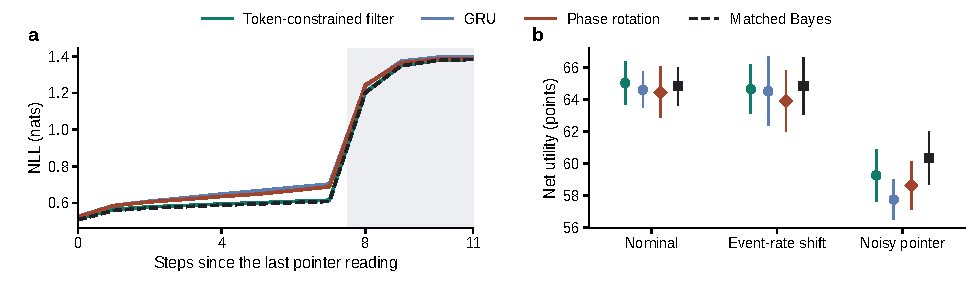
\includegraphics[width=\linewidth]{figures/feedback_results.pdf}
\caption{(a)~Nominal NLL at $L=80$ is averaged over five seeds and plotted
against steps since the last pointer reading.
Shading marks missing turns, and age zero includes the exact initial pointer
and later readings.
The dashed curve shows matched Bayes, and solid curves show the
token-constrained filter, GRU, and phase rotation.
(b)~Points show mean net utility in the nominal, event-rate shift, and
noisy-pointer regimes over $L=40,80$ and five seeds, with bars showing one
sample SD across seeds.}
\label{fig:feedback}
\end{figure}

\subsection{Planner regime sweep}
\label{app:regimes}
The sweep reuses the twenty frozen test checkpoints and the evaluation histories of the
main experiment. We vary the controller horizon $T_{\mathrm{plan}}$, the sensing
cost $c$, and the probability $\rho$ of returning the true pointer during
control. Otherwise the sensor returns a uniform token. The planner uses $\rho$
in its belief update.
Turn cost $0.04$ and turn success $0.8$ stay fixed. Action and sensor outcomes are drawn
once per cell and seed and shared by all estimators. With the original draws, $T_{\mathrm{plan}}=3$,
$c=0.08$ and $\rho=0.8$, the sweep code reproduces every per-seed utility of
Table~\ref{tab:feedback} exactly. A one-step planner never senses, and a cost of $0.4$
suppresses sensing at $\rho=0.6$, so the 75 grid points contain 53 distinct regimes.
Table~\ref{tab:regimes} shows that the cyclic filters retain the largest
minimum share of attainable utility among learned estimators.

Estimation headroom ranges from $0.3$ to $26$ points. Every learned
estimator stays within $1.5$ points of matched Bayes, and the
token-constrained filter stays within $0.66$ points. With at least ten
points of headroom, every learned estimator retains at least $89.8\%$ of
the available gain. The largest paired gain of the token-constrained
filter over the GRU is $1.47$ points.

\begin{table}[H]
\centering\small
\caption{Utility across the 75-regime planner grid. Loss to matched Bayes is
in percentage points, based on five paired seeds per regime. Retained share
uses the 40 regimes with at least ten points of headroom. Significant
losses count regimes with a seed-bootstrap interval below zero.}
\label{tab:regimes}
\begin{tabular}{lrrrrr}
\toprule
Estimator & Max loss & Mean loss & Min retained & Below uniform & Significant losses \\
\midrule
GRU & 1.47 & 0.65 & 90.1\% & 3 & 57 \\
Phase-rotation model & 1.32 & 0.63 & 89.8\% & 0 & 65 \\
Unconstrained filter & 0.66 & 0.23 & 96.6\% & 0 & 27 \\
Token-constrained filter & 0.66 & 0.21 & 95.6\% & 0 & 22 \\
Nominal Bayes & 0.73 & 0.34 & 95.4\% & 0 & 56 \\
\bottomrule
\end{tabular}
\end{table}

\FloatBarrier

\section{Recorded Inertial Sensor Protocol and Results}
\label{app:imu}

\paragraph{Data and labels.}
BROAD contains 39 trials recorded at 285.7~Hz with gyroscope, accelerometer,
and magnetometer readings and an optical reference orientation
\citep{laidig2021broad}. We use the reference only for labels. The heading is
the angle of the sensor's $x$ axis projected onto the horizontal plane. Steps
with missing optical data or pitch above $75^\circ$ are excluded from the loss
and the metrics but remain in the inputs. Averaging the IMU over blocks of ten
samples gives 28.6~Hz. The test split contains trials 02, 05, 07, 09, 11,
14, 16, 18, 20, 23, 25, 27, 29, 31, 33, 35, 37, and 39. Trials 03, 12, and 21
serve only for selecting the learning rate and model variant. The remaining
18 trials form the training split. Trials 28--38 contain magnetic disturbances,
and the split places 29, 31, 33, 35, and 37 in the test set.

\paragraph{Inputs.}
A complementary filter with gain $0.05$, tuned on training trials, runs
causally over each whole trial \citep{mahony2008complementary}. Its gravity
direction and the wrapped change $u_t$ of its heading join the gyroscope and
accelerometer features. Its absolute heading is not used. Task~B adds the
tilt-compensated magnetometer heading, the field norm, and the dip angle. The
frame offset between the magnetometer and optical headings is estimated on
undisturbed training trials only.

\paragraph{Models and training.}
Every learned model applies the same two-layer encoder of width 32 to the
standardized features. The input-set rotation uses $16$ complex channels with
angles $n\,u_t$ for $n=1,\dots,8$, two channels per harmonic, a learned initial
phase, and a Born readout over 16 sectors. Its readout and initial phase have
528 parameters. The encoder receives no gradient in this variant. The
learned-angle variant sets the angles to a linear function of the encoder output
initialized at the harmonic solution (2{,}480 parameters). A third variant adds a
learned scalar correction to $u_t$ (1{,}969 parameters). The GRU (hidden size
14), LSTM (12), and one-layer causal Transformer (width 16, four heads) have
3{,}664, 3{,}824, and 4{,}432 parameters. In Task~B the cyclic filter has 1{,}635
parameters and the GRU, LSTM, and Transformer have 7{,}312, 7{,}200, and 5{,}376.
All models train with per-step NLL on 10~s windows, Adam, batch size 32, and
gradient clipping at norm 1, for 6{,}000 updates in Task~A and 4{,}000 in
Task~B. The learning rate is chosen from $\{10^{-3},3\times10^{-3}\}$ by
validation NLL. Each setting uses five seeds.

\paragraph{Evaluation.}
Test windows start every 5~s. Their number is 739, 665, 558, 343, and 95 for
lengths 10, 30, 60, 120, and 240~s. All 18 test trials contribute except at
240~s. Only the three longest trials reach that length. We average seeds within each window
and then windows within each trial. Intervals resample whole test trials 10{,}000
times. VQF \citep{laidig2023vqf} runs offline on the raw 285.7~Hz data of each
window, in its 6D form for Task~A and its 9D form for Task~B.

\paragraph{Amendments.}
We fixed the protocol before any model was trained. In the first round no
learned model had a tilt estimate. All learned models had errors of
$25$--$39^\circ$ at 10~s, and the rotation with a learned angle collapsed to no
rotation. We kept this round as a negative result and added the gravity
direction and $u_t$ to the inputs of every learned model. The second round showed
the drift of learned angle corrections at 60~s and beyond. On validation trials
we traced the drift to a mean correction of $4.4\times10^{-4}$~rad per step.
We then added the input-set variant and ran it once on the test trials with the
same grid. We also added VQF as a reference. Task~B was specified before any of
its models were trained. Its first run read two feature columns in swapped
order. We discarded it and reran all Task~B models with corrected code. The
protocol specified two Transformer layers, but all reported runs use one layer.

\begin{table}[!htb]
\centering\small
\setlength{\tabcolsep}{4.5pt}
\caption{Task~A on held-out trials: heading error at the window end (degrees)
and test NLL (nats). Lower is better. Classical filters give point estimates
only.}
\label{tab:imu-a}
\begin{tabular}{lrrrrrcrrrrr}
\toprule
& \multicolumn{5}{c}{Error (deg)} && \multicolumn{5}{c}{NLL (nats)} \\
\cmidrule{2-6}\cmidrule{8-12}
Window length (s) & 10 & 30 & 60 & 120 & 240 && 10 & 30 & 60 & 120 & 240 \\
\midrule
Input-set rotation & 4.8 & 7.7 & 11.6 & 20.2 & 29.6 && 0.38 & 0.54 & 0.75 & 1.30 & 1.58 \\
Learned angle & 4.9 & 8.5 & 22.7 & 99.7 & 87.4 && 0.34 & 0.59 & 0.97 & 1.77 & 2.51 \\
Learned correction & 7.7 & 26.5 & 53.7 & 97.5 & 93.5 && 0.53 & 1.43 & 2.40 & 3.34 & 4.28 \\
GRU & 25.4 & 45.8 & 58.1 & 60.1 & 75.2 && 1.07 & 1.92 & 2.39 & 2.63 & 3.63 \\
LSTM & 23.0 & 43.5 & 53.9 & 53.6 & 73.9 && 1.00 & 1.86 & 2.37 & 2.66 & 4.13 \\
Transformer & 21.9 & 46.0 & 45.6 & 47.9 & 73.7 && 0.99 & 2.78 & 3.76 & 4.26 & 6.64 \\
\midrule
Integrated $u_t$ & 4.5 & 7.1 & 12.3 & 21.5 & 31.0 && \multicolumn{5}{c}{---} \\
Complementary filter & 6.9 & 9.1 & 13.8 & 22.5 & 31.4 && \multicolumn{5}{c}{---} \\
VQF (6D) & 4.2 & 6.0 & 7.7 & 6.8 & 20.7 && \multicolumn{5}{c}{---} \\
\bottomrule
\end{tabular}
\end{table}

\begin{table}[!htb]
\centering\small
\caption{Task~A paired differences, input-set rotation minus the comparison
(negative favors the input-set rotation), with 95\% trial-bootstrap intervals.
The best network is chosen per length and metric.}
\label{tab:imu-contrast}
\setlength{\tabcolsep}{4pt}
\begin{tabular}{rlrrrr}
\toprule
& & \multicolumn{2}{c}{vs.\ best network} & \multicolumn{2}{c}{Error (deg) vs.\ classical} \\
\cmidrule(lr){3-4}\cmidrule(lr){5-6}
Length (s) & Best network & Error (deg) & NLL (nats) & Integrated $u_t$ & VQF (6D) \\
\midrule
10 & Transformer & $-17.1$ [$-23.6$, $-11.3$] & $-0.62$ [$-0.83$, $-0.42$] & $+0.4$ [$+0.1$, $+0.6$] & $+0.6$ [$+0.4$, $+0.9$] \\
30 & LSTM & $-35.8$ [$-48.6$, $-23.1$] & $-1.32$ [$-1.69$, $-0.95$] & $+0.6$ [$+0.2$, $+1.1$] & $+1.7$ [$+1.2$, $+2.3$] \\
60 & Transf./LSTM & $-34.0$ [$-48.7$, $-19.3$] & $-1.61$ [$-2.11$, $-1.10$] & $-0.8$ [$-1.4$, $-0.2$] & $+3.8$ [$+2.6$, $+5.3$] \\
120 & Transf./GRU & $-27.7$ [$-44.2$, $-10.5$] & $-1.33$ [$-1.85$, $-0.78$] & $-1.3$ [$-2.3$, $-0.4$] & $+13.4$ [$+9.3$, $+17.2$] \\
240 & Transf./GRU & $-44.1$ [$-65.5$, $-31.4$] & $-2.05$ [$-2.67$, $-1.46$] & $-1.4$ [$-2.0$, $-0.6$] & $+9.0$ [$+6.9$, $+11.0$] \\
\bottomrule
\end{tabular}
\end{table}

\begin{table}[!htb]
\centering\small
\setlength{\tabcolsep}{4.5pt}
\caption{Task~B tracking error (degrees, averaged over valid steps) and test
NLL (nats) on magnetically disturbed (5) and undisturbed (13) test trials.
Classical filters give point estimates only.}
\label{tab:imu-b}
\begin{tabular}{lrrrrcrrrrcrr}
\toprule
& \multicolumn{4}{c}{Disturbed, error} && \multicolumn{4}{c}{Undisturbed, error} && \multicolumn{2}{c}{NLL, 60~s} \\
\cmidrule{2-5}\cmidrule{7-10}\cmidrule{12-13}
Window length (s) & 10 & 30 & 60 & 120 && 10 & 30 & 60 & 120 && Dist. & Undist. \\
\midrule
Cyclic filter (ours) & 9.0 & 8.9 & 9.5 & 8.9 && 5.9 & 6.0 & 6.1 & 6.1 && 2.64 & 2.57 \\
GRU & 9.9 & 11.0 & 12.6 & 11.5 && 5.5 & 5.9 & 6.2 & 6.2 && 2.67 & 1.99 \\
LSTM & 8.8 & 9.7 & 10.9 & 10.2 && 5.6 & 6.1 & 6.4 & 6.4 && 2.46 & 1.86 \\
Transformer & 9.2 & 11.9 & 15.8 & 18.0 && 5.0 & 6.7 & 8.7 & 10.9 && 3.20 & 3.40 \\
\midrule
Complementary filter & 10.8 & 9.5 & 9.2 & 8.4 && 7.2 & 7.2 & 7.3 & 7.3 && \multicolumn{2}{c}{---} \\
With rejection & 11.5 & 12.1 & 12.1 & 8.8 && 7.0 & 7.2 & 7.5 & 7.4 && \multicolumn{2}{c}{---} \\
VQF (9D) & 5.2 & 4.0 & 3.4 & 2.6 && 2.2 & 2.2 & 2.1 & 2.0 && \multicolumn{2}{c}{---} \\
\bottomrule
\end{tabular}
\end{table}

In Task~B the cyclic filter's belief update uses a learned von Mises pointer
likelihood with an outlier weight, and a learned diffusion of the shifted
belief. The criterion fixed in advance asked it to beat both the best network
and the tuned rejection filter on disturbed trials with intervals excluding
zero. At 60~s the differences are $-1.4^\circ$ $[-3.4,0.6]$ against the LSTM and
$-2.6^\circ$ $[-6.5,1.3]$ against the rejection filter, so the criterion is not
met. On undisturbed trials the filter is $1.2$--$1.4^\circ$ more accurate than
both complementary filters, with intervals excluding zero, and ties the GRU.


\end{document}
